%%%%%%%%%%%%%%%%%%%%%%%%%%%%%%%%%%%%%%%%%%%%%%%%%%%%%%%%%%%%%%%%%%%%%%%% Journal submission
%%%%%%%%%%%%%%%%%%%%%%%%%%%%%%%%%%%%%%%%%%%%%%%%%%%%%%%%%%%%%%%%%%%%%%%% SAMPLE LaTeX SOURCE (with no warranty)

\documentclass[a4paper,11pt]{elsarticle}
\usepackage{graphicx}		% include graphics
\usepackage{url}
\usepackage[utf8]{inputenc}  	% for czech diacritics (used mainly in names)
%\usepackage[latin2]{inputenc}	% if utf8 is not working correctly
%\usepackage[colorlinks=false]{hyperref} 	% hyperref support
%\usepackage{lineno}
%\linenumbers
%\usepackage{ulem}
\usepackage{subcaption}
\usepackage{float}
\usepackage{multirow}
%\usepackage{wrapfig}
\usepackage{amsmath}
\usepackage{natbib}
%\usepackage[labelfont=bf]{caption}

\usepackage[usenames,dvipsnames]{color}
\newcommand{\IF}[1]{\textcolor{red}{#1}}
\newcommand{\MP}[1]{\textcolor{blue}{#1}}
\newcommand{\MC}[1]{\textcolor{magenta}{#1}}

\makeatletter
\def\convertto#1#2{\strip@pt\dimexpr #2*65536/\number\dimexpr 1#1}
\makeatother

\journal{Neural Networks}

%%%%%%%%%%%%%%%%%%%%%%%%%%%%%%%%%%%%%%%%%%%%%%%%%%%%%%%%%%%%%%%%%%%%%%%% THE BEGINNING
\begin{document}
\begin{frontmatter}
\date{}

\title{Exploration by self-supervised exploitation}

\author[1,*]{Matej Pech\'a\v{c}}
\author[2]{Michal Chovanec}
\author[1]{Igor Farka\v{s}}

\address[1]{Department of Applied Informatics, Comenius University, Bratislava, Slovak Republic}
\address[2]{Photoneo, Ltd., Bratislava, Slovak Republic}
\address[*]{Correspondence: matej.pechac@fmph.uniba.sk}


%\ead{\{matej.pechac,igor.farkas\}@fmph.uniba.sk, mchovanec@photoneo.com}
%Photoneo Ltd. \\ 

%%%%%%%%%%%%%%%%%%%%%%%%%%%%%%%%%%%% 
\begin{abstract}
Reinforcement learning can solve decision-making problems and train an agent to behave in an environment according to a predesigned reward function. However, such an approach becomes very problematic if the reward is too sparse and the agent does not come across the reward during the environmental exploration. The solution to such a problem may be in equipping the agent with an intrinsic motivation, which will provide informed exploration, during which the agent is likely to also encounter external reward. Novelty detection is one of the promising branches of intrinsic motivation research. We present Self-supervised Network Distillation (SND), a class of internal motivation algorithms based on the distillation error as a novelty indicator, where the target model is trained using self-supervised learning. We adapted three existing self-supervised methods for this purpose and experimentally tested them on a set of ten environments that are considered difficult to explore. The results show that our approach achieves faster growth and higher external reward for the same training time compared to the baseline models, which implies improved exploration in a very sparse reward environment.~\footnote{The source code is available at \url{https://github.com/Iskandor/MotivationModels} and \url{https://github.com/michalnand/reinforcement_learning}}
~\footnote{Video of our trained agents is available at \url{https://youtu.be/-vDg_r2ZetI}}
\end{abstract}

\begin{keyword}
reinforcement learning; intrinsic motivation; self-supervised learning; knowledge distillation; hard exploration
\end{keyword}
\end{frontmatter}

%%%%%%%%%%%%%%%%%%%%%%%%%%%%%%%%%%%%%%%%%%%%%%%%%%%%%%%%%%%%%%%%%%%%%%% INTRO
\section{Introduction}
\label{sec:intro}

The development of reinforcement learning (RL) methods has achieved much success over the last decade, since together with advances in computer vision  \citep{krizhevsky2012imagenet,he2016deep}, it became possible to teach agents to solve various tasks, play computer games \citep{mnih2013playing} (see overview in \citep{RLgames2023}) even surpassing human players \citep{mnih2015humanlevel}.
Nevertheless, these single tasks require very long training times and a lot of computational resources.
Coping with complex (continuous) environments such as real world is still a challenge. There are several research opportunities, one of them being the search for more efficient learning methods.
Another is hardware development, which attempts to adapt to the requirements of neural networks that are currently being used in the RL field.

The complex environments with sparse rewards pose a special challenge for RL approaches.
The most popular computational approach to make RL more efficient is based on a concept of {\it intrinsic motivation} (IM) \citep{baldassarre2014intrinsic}. 
IM has a strong biological basis  \citep{Ryan00,Morris2022} since it is observed among higher animals, especially in humans, engaging them in various activities. 
Intrinsic motivations appear early in life and guide the biological agents during their entire life. IM is considered one of the prerequites for open-ended (or, life-long) learning. 
If we want to achieve this capacity with artificial agents \citep{Parisi2019}, we have to master this first step and equip them with an ability to generate their own goals and acquire new skills. 
Therefore, computational approaches concerned with IMs and open-ended development provide the potential in this direction leading to more intelligent systems, in particular those capable of improving their own skills and knowledge autonomously and indefinitely \citep{baldassarre2014intrinsic,Baldassarre19}.

The concept of intrinsic (and extrinsic) motivation was first studied in psychology \citep{Ryan00}, and later it entered the RL literature \citep{barto2005intrinsic, singh2010intrinsically, Barto2013}. The first taxonomy of computational models appeared in \cite{oudeyer2009intrinsic} where the concept of motivation is divided into external and internal, depending on the mechanism that generates motivation for the agent. \textit{External} motivation assumes the source of motivation coming from outside the agent and it is always associated with a particular goal in the environment. If the motivation is generated within the structures that make up the agent, this implies an \textit{internal} motivation. 

Another dimension for the differentiation, extrinsic or intrinsic, is less obvious (see also \citep{Morris2022}).
\textit{Extrinsic} motivations pertain to behaviors whenever an activity is done in order to attain some separable outcome. Some variability exists in this context, since these behaviors can vary in the extent to which they represent self-determination (see the details in \citep{Ryan00}).
On the other hand, \textit{intrinsic} motivation is defined as doing an activity for its inherent satisfaction rather than for some separable consequence (or instrumental value). It has been operationally defined in various ways, backed up by different psychological theories, which point to some uncertainty in what IM exactly means. Nevertheless,
\citep{Baldassarre19} offers a solution of an operational definition of IMs as processes that can drive the acquisition of knowledge and skills in the absence of extrinsic motivations. Furthermore, the author proposes (and explains why) a new term of \textit{epistemic motivations} as a suitable substitution for intrinsic motivations. 
Despite some uncertainty, intrinsic motivation has remained a well coined term in the literature.

Intrinsic motivation is a crucial factor that helps the agent not only to remain in open-ended learning hence solving different tasks \citep{Parisi2019}, but it also helps
to solve single difficult tasks with extremely sparse rewards. In this paper, we focus on this case.

There exists a variety of approaches aiming to use IM-based signal for agent learning. Information-theoretic view on IM is well represented in the literature,  involving the concepts of novelty, surprise and skill-learning. The recent review \citep{Aubret2023} suggests that novelty and surprise can assist the building of a hierarchy of transferable skills which abstracts dynamics and makes the exploration process more robust. In this context, abstraction is a key feature of the agent's architecture where it makes sense to introduce learning mechanisms to enforce formation of proper internal representations that lead to improved agent's performance. 

Learning the proper internal representations from unlabelled input data (e.g.~images) for the purpose of solving various problems is in general a useful task in machine learning. This can be achieved in various ways (related methods are mentioned in Sec.~\ref{sec:related-work}), including supervised end-to-end (deep) learning, self-supervised autoencoders, unsupervised feature extractors (such as contrastive divergence learning) and RL-based approaches where a certain loss function is optimized.
In our work, we focus on self-supervised approaches exploiting the novelty detection signal in feature domain to enhance RL agent's exploration.

The paper is organized as follows. In the remaining part of Sec.~\ref{sec:intro} we present the original contribution of this work. Section~\ref{sec:related-work} contains related work. Section~\ref{sec:methods} describes the methods used in this work. Section~\ref{sec:exper} explains in detail all experiments performed. Section~\ref{sec:discussion} concludes the paper with the discussion.

\subsection{The paper contribution}
We introduced and tested a class of motivational models based on the exploitation of the distillation error as novelty detection. The first such model was the Random Network Distillation model \cite{burda2018exploration}, which became the basis of our models. However, random distilled features are not the best representation, since this leads to stacking or slow convergence. Instead of distilling random features, we proposed to distil the self-supervised latent space representations. 

\begin{figure*}[thb]
\centering
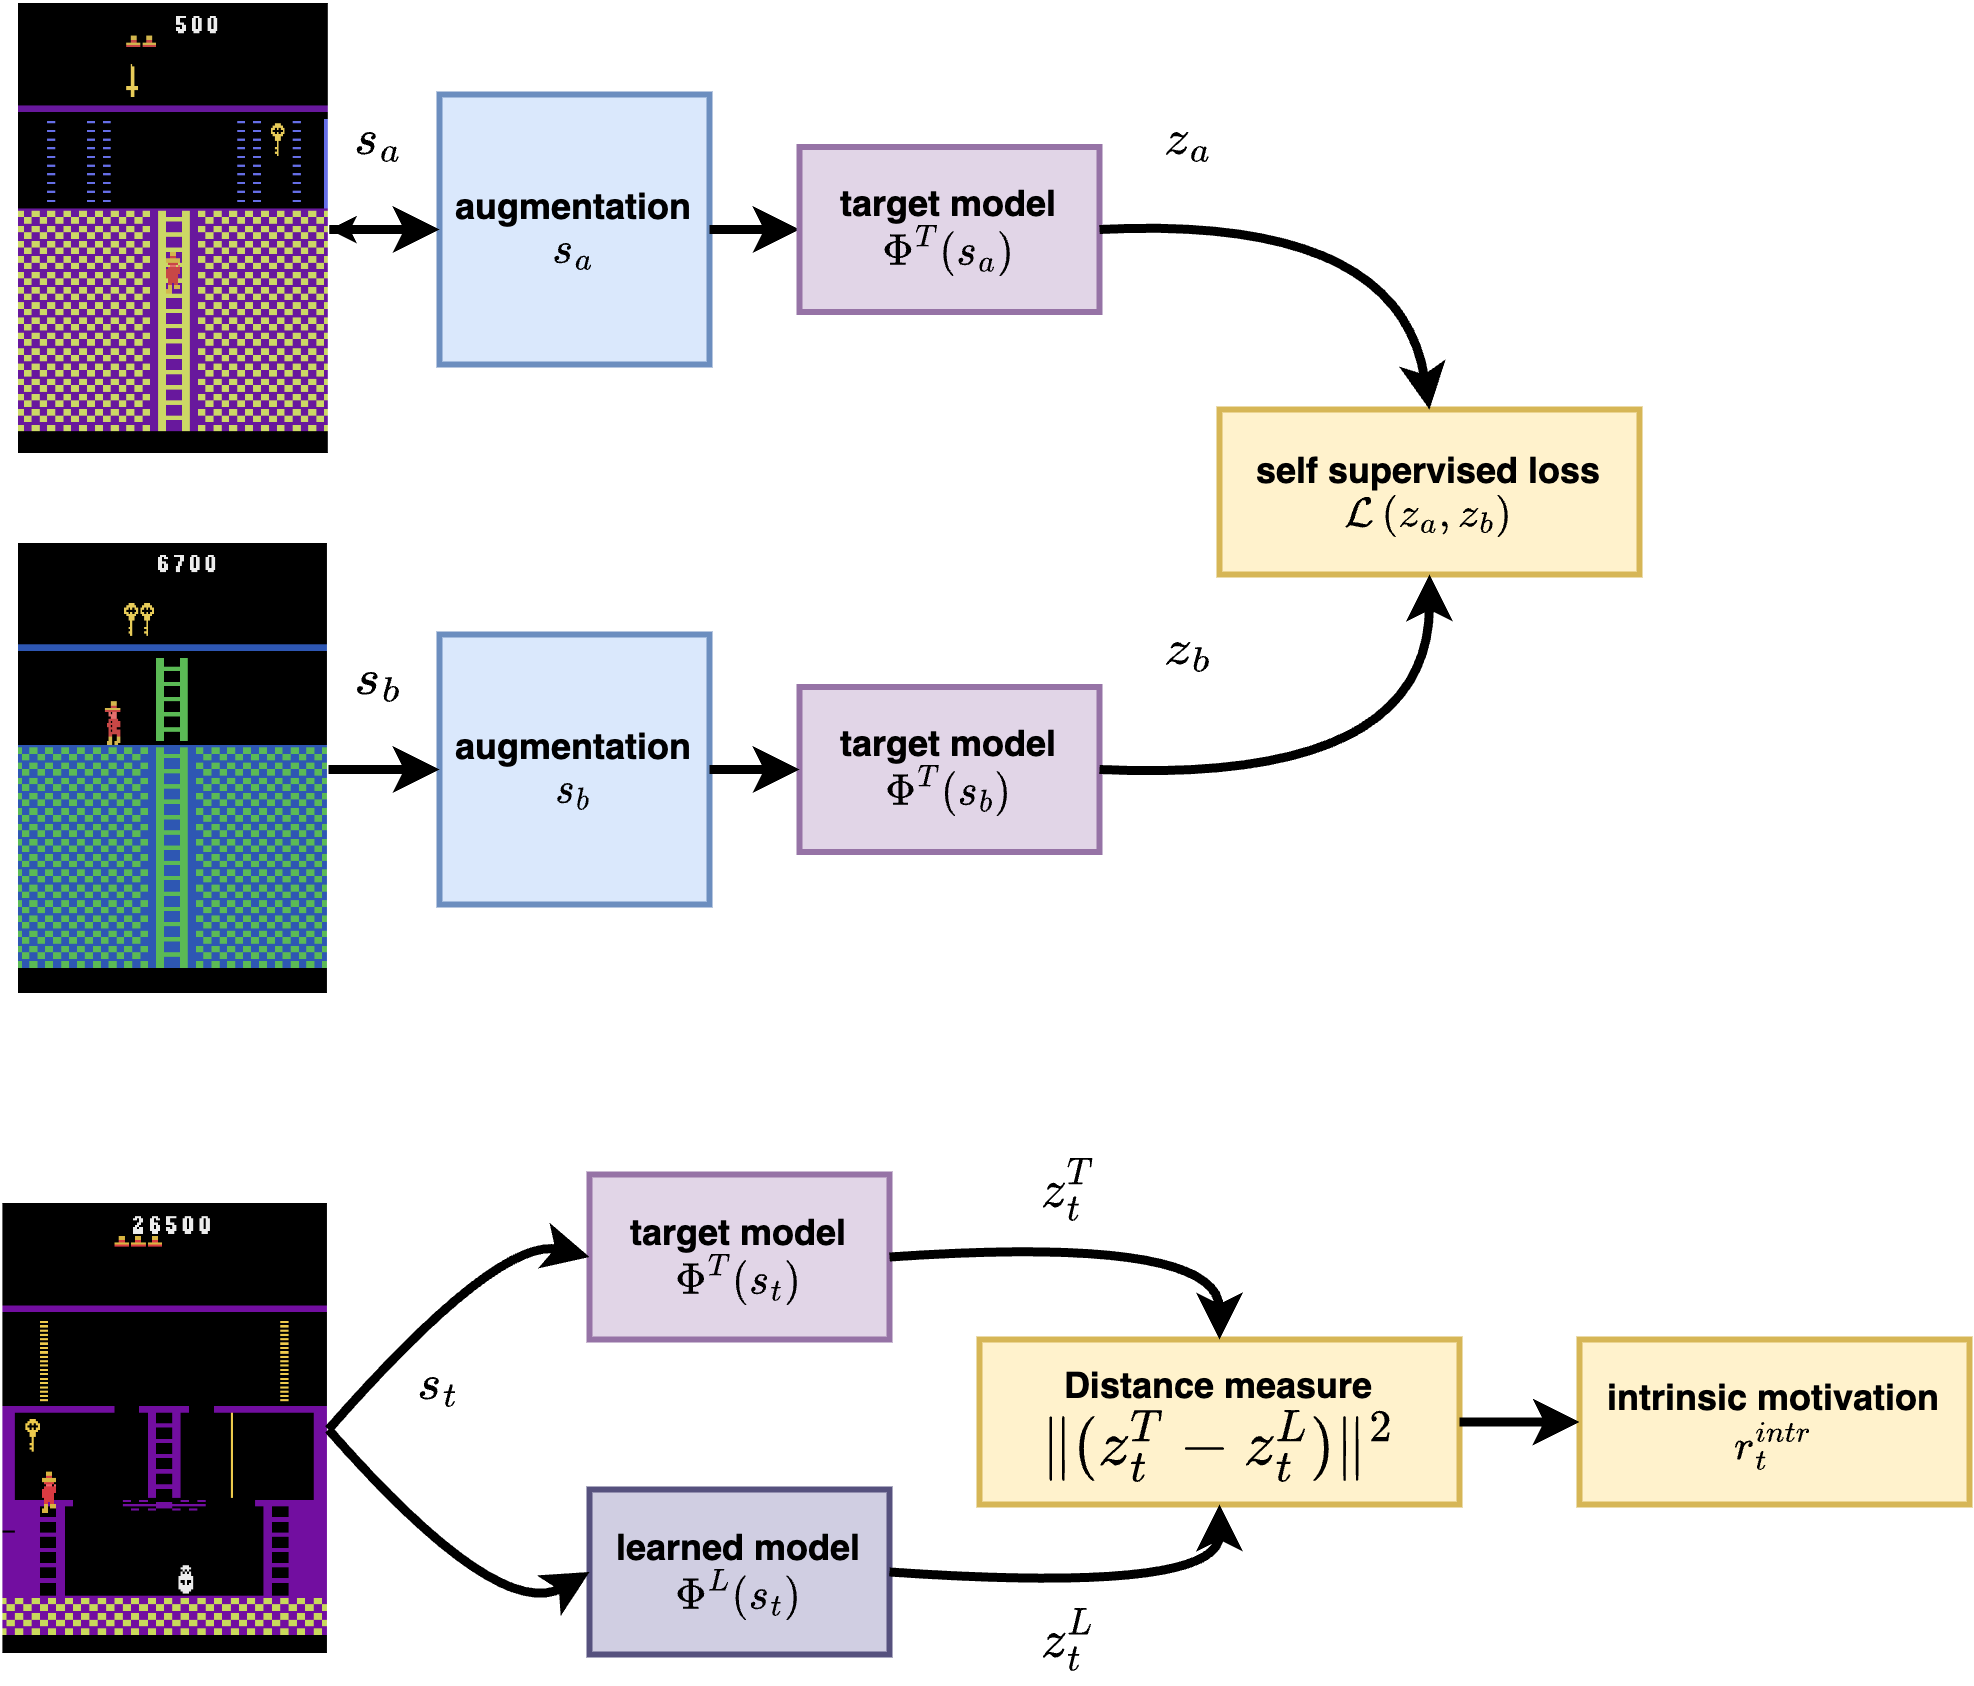
\includegraphics[width=0.8\textwidth]{fig/diagrams/cnd-overview.png}
\caption{Self-supervised network distillation (SND) principle. The proposed method consists of two main parts. {\it Top:} Self-supervised learning of the suitable features for the target model. {\it Bottom:} Calculation of the intrinsic reward by target model distillation, using the squared Euclidean distance between the models' outputs.}
\label{fig:cnd_overview}
\end{figure*}

The overall concept is shown in Fig.~\ref{fig:cnd_overview}.
Our method uses two models, one providing target features $z_{t}^{\rm T}$, called the target model $\Phi^{\rm T}(s_t)$, and the learned model $\Phi^{\rm L}(s_t)$, providing features $z_{t}^{\rm L}$. Both models use the state (observation) $s_t$ at time step $t$ as their input. 
The learned model attempts to imitate the target model, and their difference is used for internal motivation as provided in \cite{burda2018exploration}.
We asked ourselves the following questions: Are the features provided from the original random model $\Phi^{\rm T}(s_t)$ sufficient? Can we provide better features? In Random Network Distillation paper \citep{burda2018exploration}, the orthogonal weight initialization method was used to set $\Phi^{\rm T}(s_t)$ and spread out $z_{t}^{\rm T}$ across the state space, which provides sustainable intrinsic reward.
We used self-supervised regularization of $\Phi^{\rm T}$ to provide features with higher variance, and better sensitivity for novelty detection. 
The states are randomly sampled from the buffer and used for learning $\Phi^{\rm T}$. 
For sampling the states, we used two approaches
\begin{enumerate}
    \item sample one state with two different augmentations
    \item sample two consecutive states
\end{enumerate}
Simultaneously, the distillation proceeds with the learning model $\Phi^{\rm L}$ using MSE loss.
All models are trained in the same loop as the policy and the value models.
We experimented with different self-supervised losses (MSE, ST-DIM \cite{Anand2019} and VICReg \cite{Bardes2022}), covering both contrastive and non-contrastive approaches.
With these methods, we were able to solve hard exploration seeds for Procgen and the complete  first level in infamous Atari game Montezuma's revenge.

%%%%%%%%%%%%%%%%%%%%%%%%%%%%%%%%%%%%%%%%%%%%%%%%%%%%%%%%%%%%%%%%%%%%%% CHAPTER 2
\section{Related work}
\label{sec:related-work}

According to the prevailing view, the approaches to IM can be divided into two main categories with adaptive motivations.
\textit{Knowledge-based} approach is focused on acquisition of knowledge of the world and it draws on the theory of drives, theory of cognitive dissonance and optimal incongruity theory. \textit{Competence-based} approach focuses on acquisition of skills by motivating the agent to achieve a higher level of performance in the environment, which means to acquire desired actions to achieve self-generated goals. Its psychological basis includes the theory of effectance and the theory of flow. 

The knowledge-based category focusing on exploration can be divided into \textit{prediction-based}, \textit{novelty-based} and \textit{information-based} approaches \citep{aubret2019survey}.
Prediction-based approaches use prediction error as an intrinsic reward signal. The source of error can be a forward model (e.g. \cite{stadie2015incentivizing,bellemare13arcade,Pathak2017}), a generative model \cite{yu2020intrinsic} (e.g. based on a variational auto-encoder \cite{kingma2013auto}) or disagreement in learned world model \citep{sekar2020planning}. Exploration with Mutual Information (EMI) \citep{kim2018emi} extracts predictive signals that can be used to guide exploration based on forward prediction in the representation space. Model-Based Active eXploration (MAX) \citep{shyam2019model} uses an ensemble of forward models to plan observing novel events.

The novelty-based approaches monitor the state novelty and the intrinsic signal is based on its value. The first models were based on count-based approach \citep{tang2017exploration}. This method is impractical for large or continuous state spaces and it was extended by introducing pseudo-count and neural density models \citep{ostrovski2017count,martin2017count,machado2018count}. A similar method to pseudo-count was used by a random network distillation (RND) model \citep{burda2018exploration} with a lower complexity. Never-give-up framework \citep{badia2020never} learns intrinsic rewards composed of episodic and life-long state novelty (which is detected by RND model).

Information approaches use quantities from information theory \citep{shannon1948mathematical}, such as information gain, mutual information, entropy and try to maximize the information obtained by the agent from the environment. Variational Information Maximizing Exploration (VIME) \citep{houthooft2016vime} approximates the environment dynamics, uses the information gain of the learned dynamics model as intrinsic rewards. Random Encoders for Efficient Exploration (RE3) \citep{seo2021state} is an exploration method that utilizes state entropy as an intrinsic reward.
For more details we recommend surveys \cite{burda2018large, aubret2019survey, yuan2022intrinsically}.

Self-supervised learning is a paradigm of machine learning, when the agent does not have any labeling of the data, but generates it on its own. The goal is to use the information in the data itself and prepare the model to perform another task. Self-supervised learning also started to be used in the field of state representation learning \citep{Timoth2018} it is proving to be a suitable method for creating the feature space \citep{Anand2019} and has also found its use in reinforcement learning \citep{Srinivas2020, guo2022byol}. Contrastive learning \citep{Chopra2005} is a method of self-supervised learning used to learn the general features by teaching the model which data points are similar or different. Several different objective functions were proposed, e.g. Noise Contrastive Estimation (NCE) \citep{Gutmann2010}, InfoNCE \citep{Oord2018}, or multi-class $N$-pair loss \citep{Sohn2016}. Another method of self-supervised learning is based on regularization (non-contrastive methods). In this case, the model sees only positive examples and generates a feature space based on various regularization losses like invariance and covariance loss in the case of Barlow Twins model \citep{Zbontar2021}, triple variance-invariance-covariance losses in VICReg model \citep{Bardes2022} or other priors like proportionality, variability, slowness principle, or repeatability \citep{jonschkowski2015learning}. 
Bootstrap Your Own Laten (BYOL) \citep{grill2020bootstrap} relies on two neural networks, referred to as online and target networks, that interact and learn from each other.

%%%%%%%%%%%%%%%%%%%%%%%%%%%%%%%%%%%%%%%%%%%%%%%%%%%%%%%%%%%%%%%%%%%%%%%% CHAPTER 3
\section{Methods}
\label{sec:methods}

The decision making problem in the environment using RL is formalized as a Markov decision process which consists of a state space $\mathcal{S}$, action space $\mathcal{A}$, transition function $\mathcal{T}_{s,a,s'} = p(s_{t+1} = s'|s_t = s, a_{t} = a)$, reward function $\mathcal{R}_{sas'}$ and a discount factor $\gamma$. The main goal of the agent is to maximize the discounted return  
$R_t = \sum_{k=0}^\infty \gamma^k r_{t+k}$
in each state, where $r_t$ is immediate external reward at time $t$.
Stochastic policy is defined as a state dependent probability function $\pi : \mathcal{S} \times \mathcal{A} \rightarrow [0, 1]$, such that
$\pi_{t}(s,a) = p(a_t = a | s_t = s)$ and $\sum_{a \in \mathcal{A}} \pi(s,a) = 1$
and the deterministic policy $\pi: \mathcal{S}\rightarrow \mathcal{A}$ is defined as $\pi(s) = a$.

An agent following the optimal policy $\pi^{*}$ maximizes the expected return $R$. The methods searching for the optimal policy can be divided into on-policy (family of actor--critic algorithms), e.g.~\cite{schulman2017proximal}
and off-policy methods (family of Q-learning algorithms), e.g.~\cite{mnih2013playing}.
Actor--critic algorithms are based on two separate modules: an \textit{actor} generates actions following the agent's policy $\pi$ and a \textit{critic} estimates the state value function $V^{\pi}$ defined as
$$
V^{\pi}(s) = \sum_a \pi(s,a) \sum_{s'} \mathcal{T}_{s,a,s'} \left[ \mathcal{R}_{s,a,s'} + \gamma V^{\pi}(s') \right]
$$
or the state-action value function $Q^{\pi}$ defined as
$$
Q^{\pi}(s,a) = \sum_{s'} \mathcal{T}_{s,a,s'} \left[ \mathcal{R}_{s,a,s'} + \gamma V^{\pi}(s') \right]
$$
The actor then updates its policy to maximize return $R$ based on critic's value function estimations.

In high-dimensional tasks, when one cannot use the Bellman equation, the common approach is to use function approximators (deep convolutional neural networks) for estimating the critic and the actor.

\subsection{Intrinsic motivation and exploration}

During the learning process, the agent must explore the environment to encounter an external reward and learn to maximize it. This can be ensured by adding noise to the actions, if the policy is deterministic, or it is already its property, if the policy is stochastic. In both cases, we say that these are uninformed environmental exploration strategies. The problem arises if the external reward is very sparse and the agent cannot use these strategies to find the sources of reward. In such a case, it is advantageous to use informed strategies, which include the introduction of intrinsic motivation.

In the context of RL, intrinsic motivation can be realized in various ways, but most often it is a new reward signal $r^{\rm intr}_t$ scaled by parameter $\eta$, which is generated by the motivational part of the model (we refer to it as the motivational module) and is added to the external reward $r^{\rm ext}_t$
\begin{equation}
\label{eq:rintr}
  r_t = r_t^{\rm ext} + \eta \, r_t^{\rm intr}
\end{equation}
The goal of introducing such a new reward signal is to provide the agent with a source of information that is absent from the environment when the reward is sparse, and thus facilitate the exploration of the environment and the search for an external reward.

%\subsection{Intrinsic motivation based on prediction error}

%Internal motivation based on the prediction error uses as a source of motivation the error of the forward model $\Psi$ whose task is to predict the next state ${s}_{t+1}$ if it receives the current state $s_t$ and the action $a_t$. The difference (e.g. MSE) between the new observed state $s_{t+1}$ and the predicted state $\hat{s}_{t+1}$ can be used as an \sout{internal} \IF{intrinsic} reward. The assumption is that the forward model will yield lower errors in states it has visited many times and, conversely, higher errors for states that were visited rarely or never. The task can be simplified so that the forward model  \IF{is trained to make predictions} \sout{predict} \sout{with}in the latent space (generated by feature extractor $\Phi$), \IF{which} \sout{thereby} eliminates the need to use a decoder that maps a point from the latent space to the state space. Instead, the difference between the latent code ${z}_{t+1}$ for ${s}_{t+1}$ and the predicted latent code $\hat{z}_{t+1}$ is used as a source of motivation $r_{\rm intr}$ defined as
%\begin{equation}
%\label{eq:prediction_error}
%r_{t}^{\rm intr} = \| \hat{z}_{t+1} - {z}_{t+1} \| ^{2}
%\end{equation}
%where $\hat{z}_{t+1} = \Psi({z}_{t}, {a}_{t})$, ${z}_{t} = \Phi(s_t)$, ${z}_{t+1} = \Phi(s_{t+1})$ and $\|.\|$ denotes the Euclidean norm. The latent space representations can be created in different ways. For example, ICM model \citep{Pathak2017} used the loss function based on the forward and inverse model.


\subsection{Intrinsic motivation based on distillation error}

In this class of methods the motivation module has two components: the target model $\Phi^{\rm T}$ that generates features (typically as a kind of feature extractor), and the learning network $\Phi^{\rm L}$ that tries to replicate them. This process is called knowledge distillation. Intrinsic motivation, expressed as an intrinsic reward, is computed as the distillation error
\begin{equation}
\label{eq:distill_error}
r_{t}^{\rm intr} = \| (\Phi^{\rm L}(s_t) - \Phi^{\rm T}(s_t)) \| ^{2}.
\end{equation}
It is assumed that the learning network will be able to more easily replicate feature vectors for states it has seen multiple times, while new states will induce a large distillation error.
The RND \citep{burda2018exploration} model shown in Fig.~\ref{fig:cnd_rnd} is a representative of this type of IM.
It is simple and successful in the environments with sparse reward but has two serious drawbacks: (1) It is necessary to properly initialize the random network; and (2) over time, the signal of intrinsic motivation disappears due to sufficient adaptation of the learning network (a phenomenon that could be called generalization).

\begin{figure*}[thb]
  \centering
  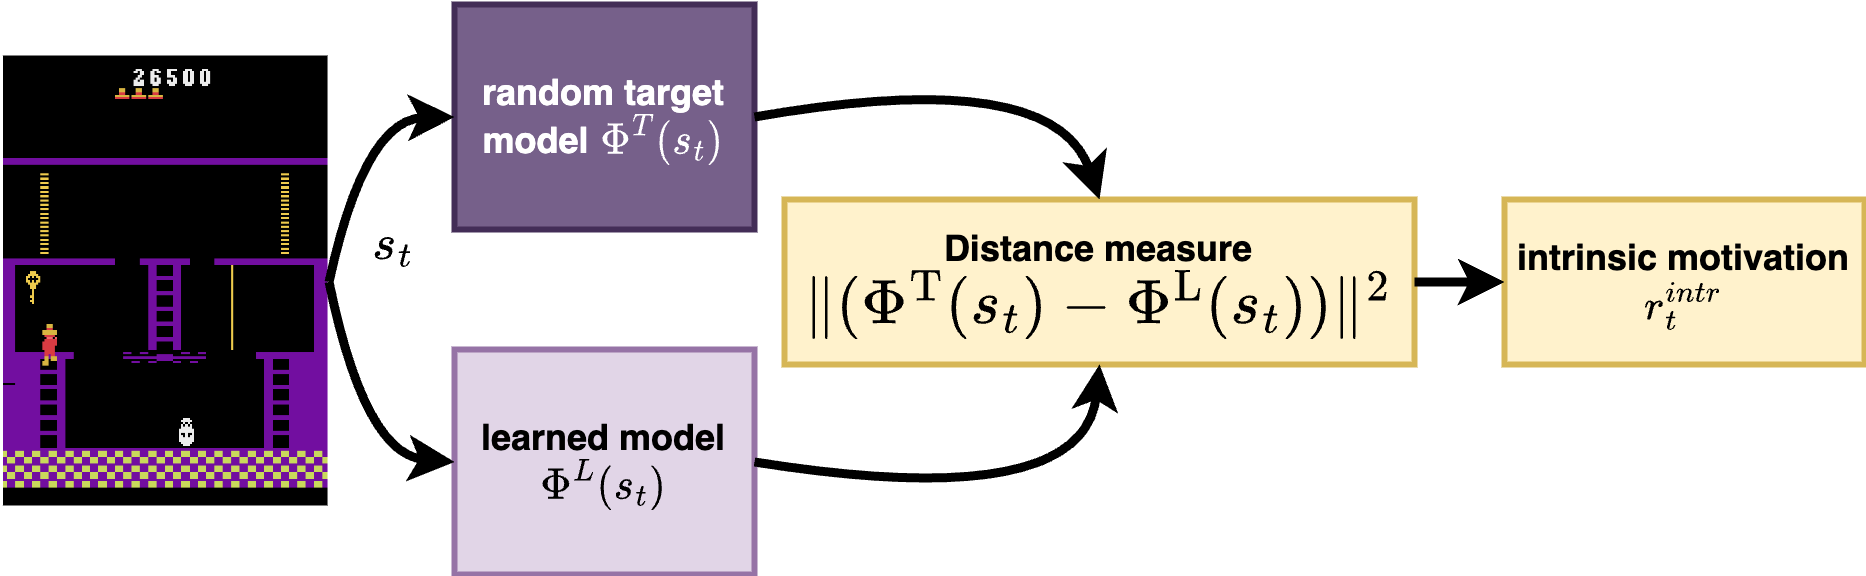
\includegraphics[width=9cm]{fig/diagrams/cnd-rnd.png}
  \caption{The basic principle of generating an exploration signal in random network distillation.}
\label{fig:cnd_rnd}
\end{figure*}

\begin{figure*}[h]
\centering
  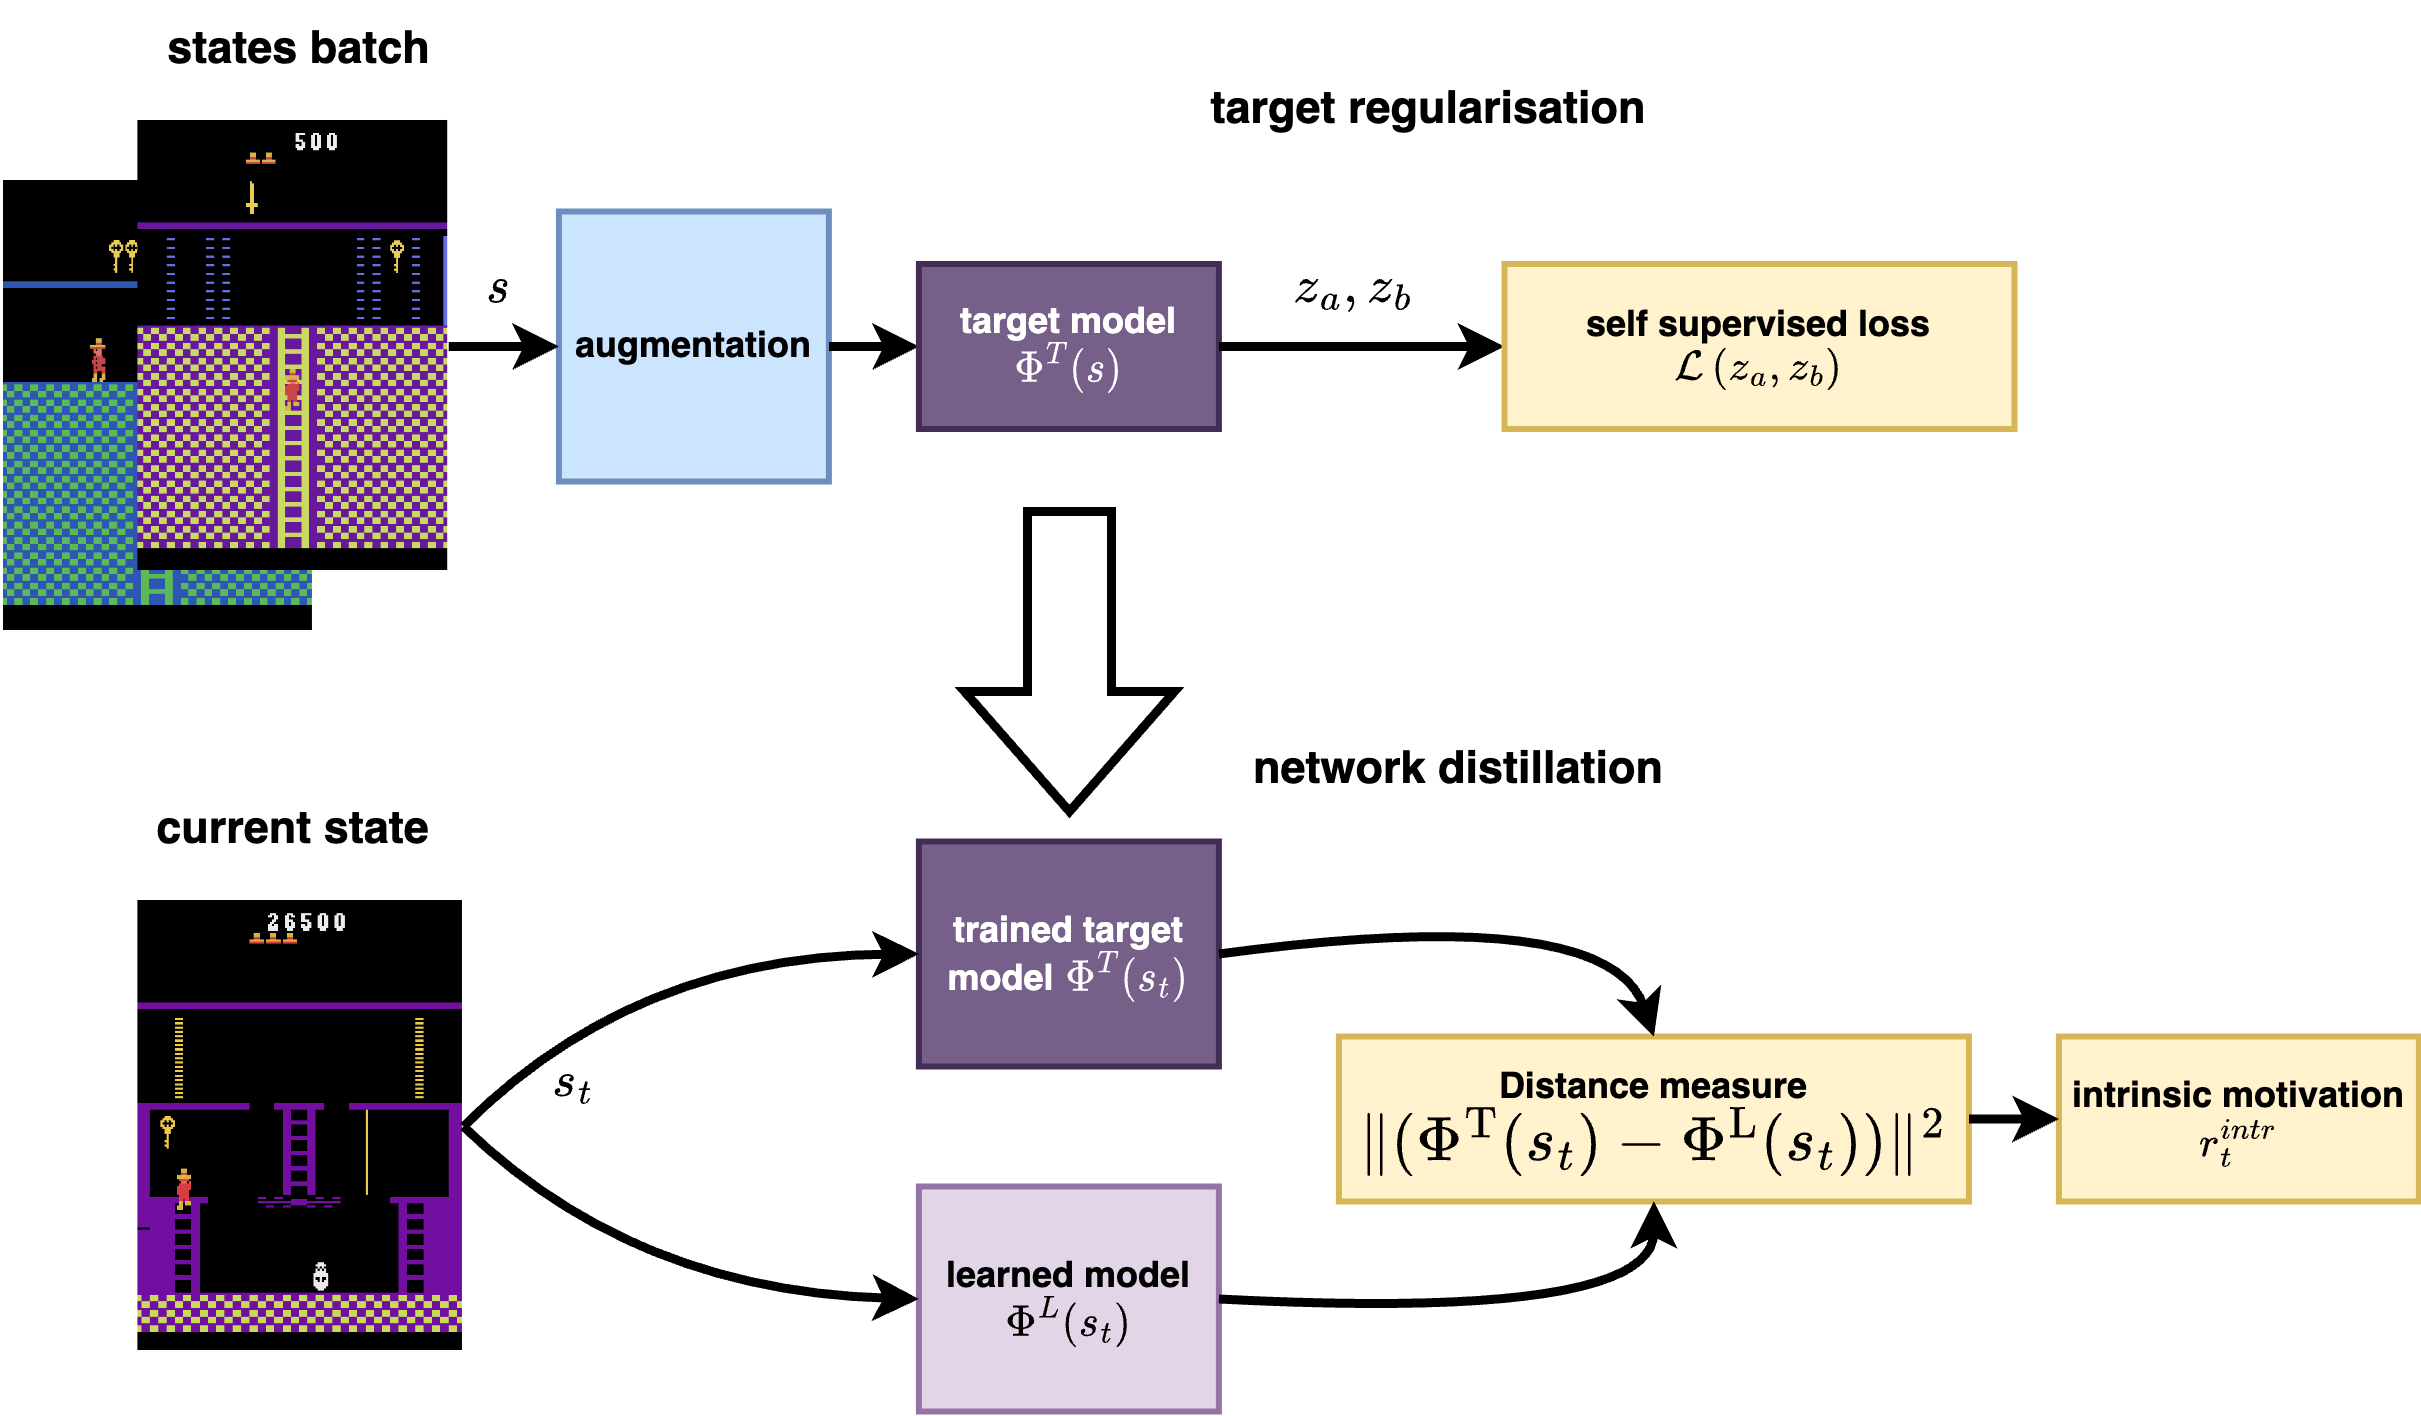
\includegraphics[width=11cm]{fig/diagrams/cnd-cnd.png}
  \caption{The basic principle of generating an exploration signal in the regularized target model, followed by RND.}
  \label{fig:cnd_cnd}
\end{figure*}

\begin{figure*}[thb]
\centering
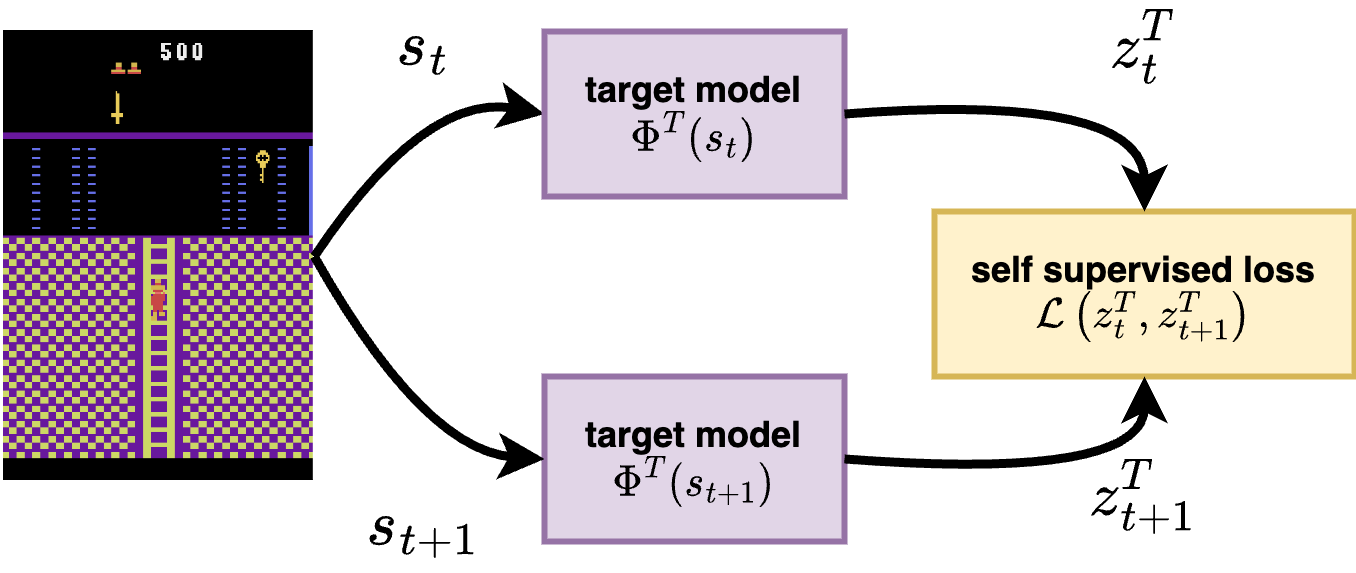
\includegraphics[width=8cm]{fig/diagrams/cnd-std.png}
\caption{Training of the SND target model using two consecutive states and the self-supervised learning algorithm.}
\label{fig:std_dim_idea}
\end{figure*}


\subsection{Self-supervised Network Distillation}

We modified the concept of distillation of randomly initialized static network RND \citep{burda2018exploration} and instead we distilled a network that learns continuously using self-supervised algorithms. We denote the methods SND. The architecture of such model consists of a target model $\Phi^{\rm T}$ and a learned model $\Phi^{\rm L}$, but with the essential difference that the network generating the target feature vectors (target model) is learned. The schematic representation of proposed approach is shown in Fig.~\ref{fig:cnd_cnd}.
In order to be able to use the trained target model as a suitable source of target feature vectors for the learning network, it is necessary that it fulfills the following conditions:
\begin{enumerate}
\item Two identical states must map to the same feature vector.
\item Two similar (e.g. successive states) are mapped on two similar feature vectors, e.g. their $L_{2}$ distance is small.
\item Two different states are mapped on two different feature vectors, e.g. their $L_{2}$ distance is large.
\end{enumerate}

The feature space formed in this way can be distilled and then this process can be used as a source of internal motivation, because the new states will have different feature vectors than the states seen by the agent so far.
We introduced three methods for forming a feature space that satisfies the above conditions. All three methods are based on self-supervised learning.

\textbf{SND-V} method (vanilla SND) uses a contrastive approach.
First the two augmented batches of states $S$, $S'$ are sampled and the corresponding feature batches $Z$, $Z'$ are computed as $\Phi^{\rm T}(s) = z$, where $s \in S, z \in Z$.
The sampling process takes with $p=0.5$ the same states.
For the same states, we set the target distance to $\tau_i = 0$, and for different states we set the distance to $\tau_i =1$.
We experimented with three augmentation schemes : 
\begin{enumerate}
    \item uniform noise only, from the range $\langle -0.2, 0.2\rangle$
    \item random tile masking + uniform noise, tiles sizes $2, 4, 8, 12, 16$
    \item random convolution filter + random tile masking + uniform noise
\end{enumerate}
Uniform noise was used for each state pixel, remaining augmentations with $p=0.5$. The whole pipeline is shown in Fig.~\ref{fig:stdv_augmentations}. 
The idea of tiles masking can be supported by recently proposed self-supervised loss \citep{assran2022maskednetworks}. Random convolution was successfully used in \citep{lee2020randomization}, for a PPO agent in Procgen environment. And finally, noise is a common augmentation process.

\begin{figure*}
\centering
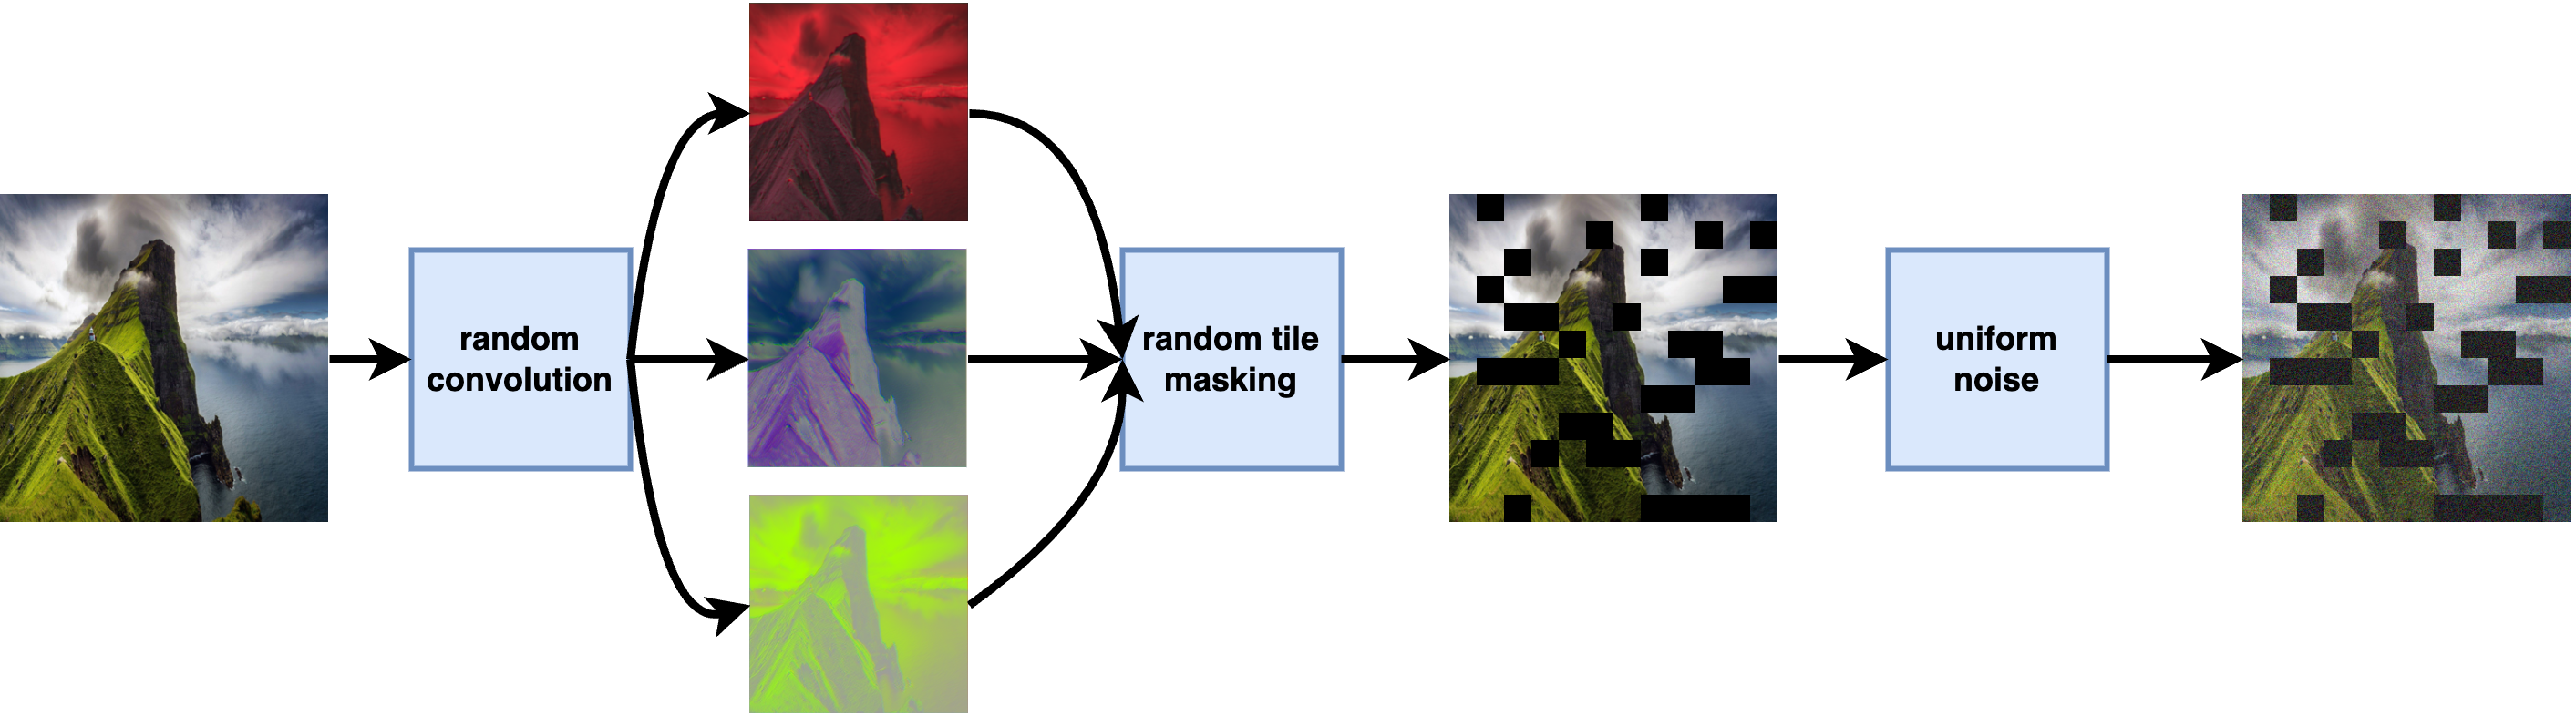
\includegraphics[width=14cm]{fig/diagrams/cnd-augmentations.png}
\caption{The scheme of the state augmentation pipeline.}
\label{fig:stdv_augmentations}
\end{figure*}

The regularisation loss is defined as
\begin{equation}
\label{eq:sndv1}
\mathcal{L} = \sum_{i}(\tau_i - \|Z_i - Z'_i\|^2_2)^2
\end{equation}
where $\|.\|^2_2$ is the squared Euclidean distance between $i-{\rm th}$ feature vectors $Z_i$ and $Z'_i$. 
We also experimented with the loss function defined as
\begin{equation}
\label{eq:sndv2}
\mathcal{L} = 
  \begin{cases}
    \|Z_i - Z'_i\|^2_2 & \text{if $\tau_i = 0$} \\
    \max(1 - \|Z_i - Z'_i\|^2_2; 0) & \text{otherwise}
  \end{cases}
\end{equation}
This loss function pulls the feature vectors of similar states (when $\tau = 0$) to one another by penalizing their squared distance. And on the contrary, it sets apart the feature vector from one another, up to a certain limit when their distance exceeds one.
However, we did not find any benefits of this loss.

\textbf{SND-STD} method uses the Spatio-Temporal DeepInfoMax (ST-DIM) algorithm \citep{Anand2019} (the simple diagram can be found in Fig.~\ref{fig:std_dim_idea}) leveraging multi-class $N$-pair losses \citep{Sohn2016}: 
\begin{equation}
\label{eq:sndstd1}
\mathcal{L}_{\rm GL} = - \sum_{i=1}^{I} \sum_{j=1}^{J} \log \frac{ \exp (g_{i,j})} { \sum_{s_{t}^{*} \in S_{\rm next}} \exp (g_{i,j})}
\end{equation}
\begin{equation}
\label{eq:sndstd2}
\mathcal{L}_{\rm LL} = -  \sum_{i=1}^{I} \sum_{j=1}^{J} \log \frac{ \exp (f_{i,j})} { \sum_{s_{t}^{*} \in S_{\rm next}} \exp (f_{i,j})}
\end{equation}
where $f(.) = f(s_t, s_{t+1})$ and $g(.) = g(s_t, s_{t+1})$
are score functions for local-local objective $\mathcal{L}_{\rm LL}$ and global-local objective $\mathcal{L}_{\rm GL}$, respectively. 
Function $g_{i,j}$ is defined as the unnormalized cosine similarity between transformed global features $\Phi^{\rm T}(s_t)$ and the local features $\Phi^{\rm T}_{(l,i,j)}(s_{t+1})$ of the intermediate layer $l$ in $\Phi^{\rm T}$, where $(i,j)$ is the spatial location. Analogically $f_{i,j}$ is the unnormalized cosine similarity between transformed local features $\Phi^{\rm T}_{(l,i,j)}(s_t)$ and $\Phi^{\rm T}_{(l,i,j)}(s_{t+1})$. The details of this algorithm are provided in \cite{Anand2019}. $S_{\rm next}$ corresponds to the set of next states, $(s_t, s_{t+1})$ represents a pair of consecutive states, $(s_t, s_{t}^{*})$ represents a pair of non-consecutive states and $I,J$ are the width and the height from output shape of intermediate convolutional layer of the target model.
The resulting loss function is then defined as
\begin{equation}
\label{eq:sndstd3}
\mathcal{L} = \frac{1}{IJ} (\mathcal{L}_{\rm GL} + \mathcal{L}_{\rm LL})
\end{equation}
Following this objective function, the target model becomes a good feature extractor adapting to new states discovered by the agent. However, after initial tests, we found that the feature space formed by such an objective function tends to grow exponentially from a certain point until it eventually explodes. We provide a more detailed analysis of this problem in Section~\ref{sec:discussion}. The solution to this problem was to find a suitable regularization that would add to the existing loss function. We decided to minimize $L_2$-norm of logits represented by functions $f$ and $g$:
\begin{equation}
\label{eq:sndstd4}
\mathcal{L}_{n} = p_{\rm GL} + p_{\rm LL} = 
\sum_{i=1}^{I} \sum_{j=1}^J (\| f_{i,j} \| + \| g_{i,j} \|)
\end{equation}
Finally, we added one more regularization term $\mathcal{L}_v$ that maximizes the standard deviation $\sigma$ of the feature vector components and thus ensures that all dimensions of the feature space are used. The analysis section provides a more detailed justification for the introduction of the given term:
\begin{equation}
\label{eq:sndstd5}
\mathcal{L}_{v} = -\sigma(\Phi^{\rm T}(s_t))
\end{equation}

The final objective function, with the scaling parameters $\beta_{1}=\beta_{2}=0.0001$ (found experimentally), was defined as
\begin{equation}
\label{eq:sndsd6}
\mathcal{L} = \frac{1}{I J} (\mathcal{L}_{\rm GL} + \mathcal{L}_{\rm LL} + \beta_{1} \mathcal{L}_{n}) + \beta_{2} \mathcal{L}_{v}
\end{equation}

\textbf{SND-VIC} method is based on VICReg algorithm \citep{Bardes2022}. The regularization function consists of three terms: the invariant term, which brings the feature vectors closer to each other, the variance term, which ensures that the feature vectors within one batch have different values, and the covariance term, which ensures the decorrelation of the feature vectors and prevents information collapse. The original method does not need any negative samples, it only takes the input, creates two augmented versions, and their feature vectors are updated using the mentioned terms of the regularization function. Our version uses the state $s_t$ and its successor $s_{t+1}$ (the same as ST-DIM, the simple diagram can be found in Fig.~\ref{fig:std_dim_idea}) instead of two augmentations of the same state.
The variance regularization term $\mathcal{L}_{v(Z)}$ is defined as a hinge function on the standard deviation of the features along the batch dimension
\begin{equation}
\label{eq:sndvic1}
\mathcal{L}_{v(Z)} = \frac{1}{d} \sum_{j=1}^{d} \max(0; \tau - \sigma(Z_j)) 
\end{equation}
where $d$ is the dimensionality of the feature space, $Z_{j}$ is $j$-${\rm th}$ feature vector from the batch $Z$, $\sigma$ is the actual standard deviation and $\tau = 1$ is a constant target value for the standard deviation. The covariance regularization term $\mathcal{L}_{c(Z)}$ is defined as the sum of the squared off-diagonal coefficients of the covariance matrix $C(Z)$
\begin{equation}
\label{eq:sndvic2}
\mathcal{L}_{c(Z)} = \frac{1}{d} \sum_{i\neq j} [C(Z)]^{2}_{i,j}
\end{equation}
The invariance criterion $\mathcal{L}_{s(Z,Z')}$ between two batches $Z$ and $Z'$ is defined as the mean-squared Euclidean distance between each pair of feature vectors
\begin{equation}
\label{eq:sndvic3}
\mathcal{L}_{s(Z, Z')} = \frac{1}{d}\sum_{i = 1}^{d}\|Z_i - Z'_i\|^2_{2}
\end{equation}
The overall loss $\mathcal{L}$ then takes the form
\begin{equation}
\label{eq:sndvic4}
\mathcal{L} = \lambda \mathcal{L}_{s(Z, Z')} + \mu \left[\mathcal{L}_{v(Z)} + \mathcal{L}_{v(Z')}\right] + \nu \left[\mathcal{L}_{c(Z)} + \mathcal{L}_{c(Z')}\right]
\end{equation}
where the scaling parameters are set to $\lambda=1$, $\mu=1$ and $\nu=1/25$.


%%%%%%%%%%%%%%%%%%%%%%%%%%%%%%%%%%%%%%%%%%%%%%%%%%%%%%%%%%%%%%%%%%%%%%%% CHAPTER 4
\section{Experiments}
\label{sec:exper}

All together, we tested our methods on 10 environments (Atari and Procgen) that are considered difficult for exploration.
These include 6 Atari environments: Montezuma's Revenge, Gravitar, Venture, Private eye, Pitfall, Solaris. The agent receives a reward of +1 for each increase in the score, regardless of its size. It does not receive any other reward or punishment. The state is represented by 4 consecutive frames of pixels on grey scale, so the dimensionality of the state representation is 4$\times$96$\times$96$\times$256. The action space is discrete, consisting of 18 actions, of which only some make sense (depending on the environment), the other actions have no impact on the environment.

We also tested 4 Procgen environments: Coinrun, Caveflyer, Jumper and Climber. Procgen is a set of procedurally generated environments, designed primarily for testing agent's generalisation \citep{cobbe2020procgen}. The paper shows several problems for generalisation in RL, requiring special training and a huge amount of samples. For our purpose, interesting findings are provided in Appendix B.1 in \citep{cobbe2020procgen}. For several seeds, the baseline agent was not able to reach a non-zero score. Those seeds lead to hard exploration environments, with only a single reward at the end. Together with fast run of these environments (thousands of FPS on single CPU core), makes Procgen good candidate for our experiments. The state is represented by RGB color images, with the size 64$\times$64 pixels. The action space is discrete, consisting of 15 actions.

Preliminary experiments were performed in \citep{pechac2022intrinsic}.

\subsection{Training setup}

We ran 9 simulations for each environment, taking 128M steps for Atari and 64M steps for Procgen games. Before the main training, we tried 3 hand-selected settings of hyperparameters for individual motivational models (mainly the scaling of the motivational signal, or regularization terms) and we always chose the one that had the best results. These short probes lasted 32M (Atari) or 16M (Procgen) steps and consisted of 2 to 3 simulations. 

All agents were trained with the PPO algorithm \citep{schulman2017proximal} using Adam algorithm \citep{kingma2015adam} to optimize the parameters of all modules. The basic agent consists of an actor and a critic, which are two multi-layer perceptrons sharing a common convolutional neural network (CNN) that processes the video input. The critic has two outputs (heads), one for estimating the value function for the external reward and the other for the internal reward. We used the orthogonal weight initialisation with a magnitude $\sqrt{2}$. 
Model architectures are presented in Figures \ref{img:ppo_arch} to %\ref{img:cnd_target_arch}, 
\ref{img:cnd_learned_arch}. 
The motivational module consists of two CNNs (the target and the learning network), which receive input from a single frame. The learning network has two more linear layers to have an increased capacity over the target model. 

\begin{figure*}[t!]
\centering
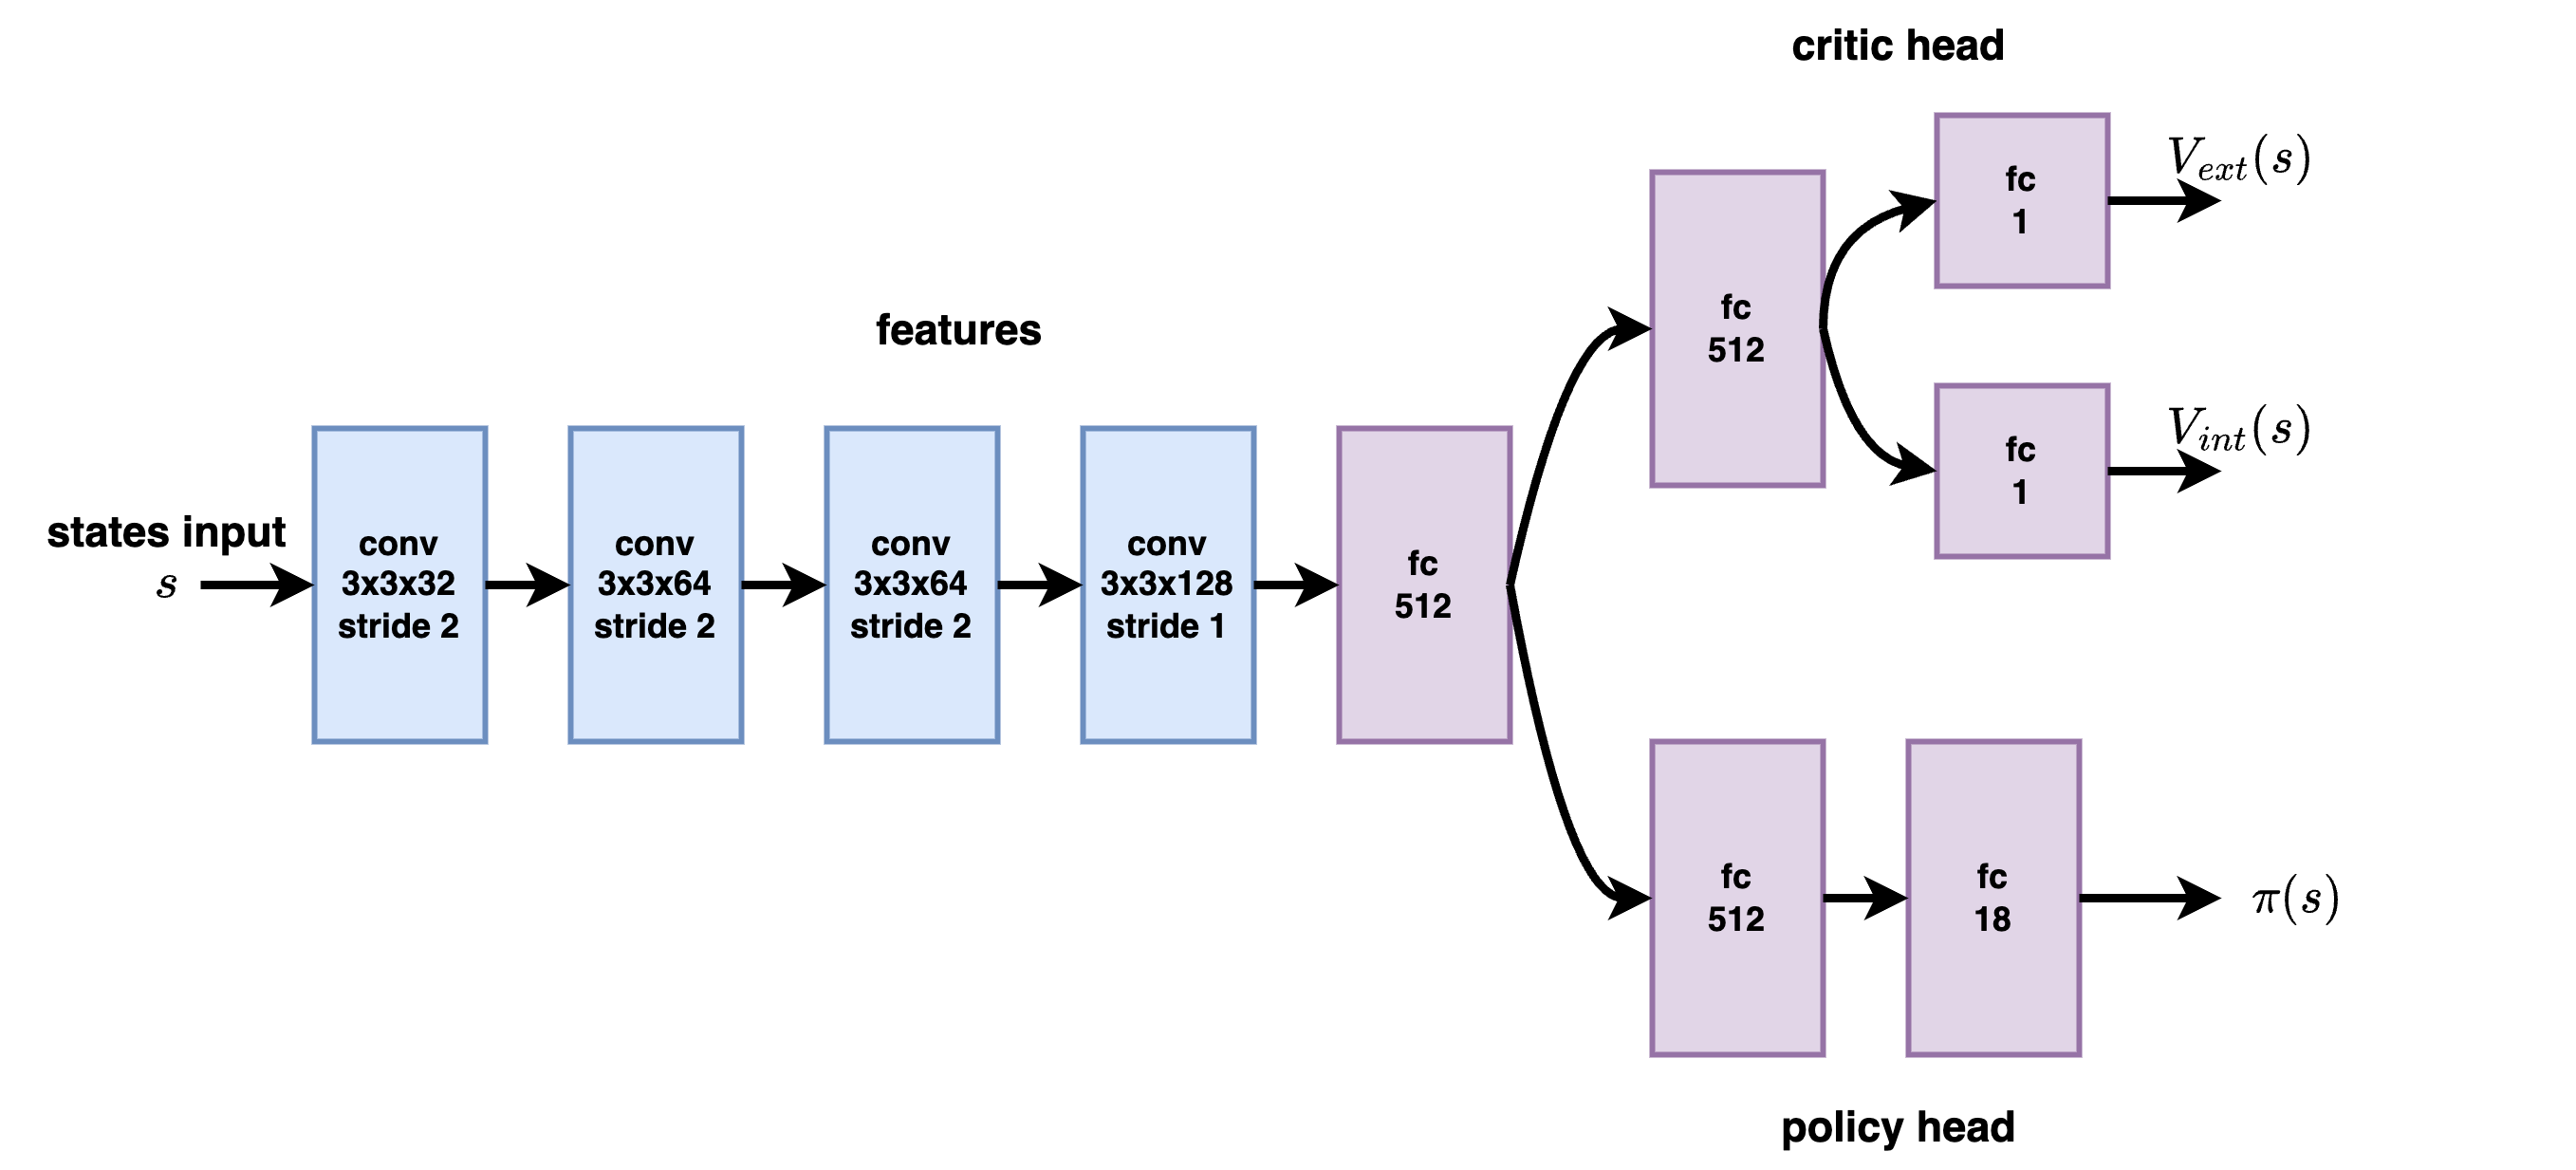
\includegraphics[width=13cm]{fig/diagrams/cnd-ppo_model.png}
\caption{The PPO agent model architecture.}
\label{img:ppo_arch}
\end{figure*}
\begin{figure*}[t!]
\centering
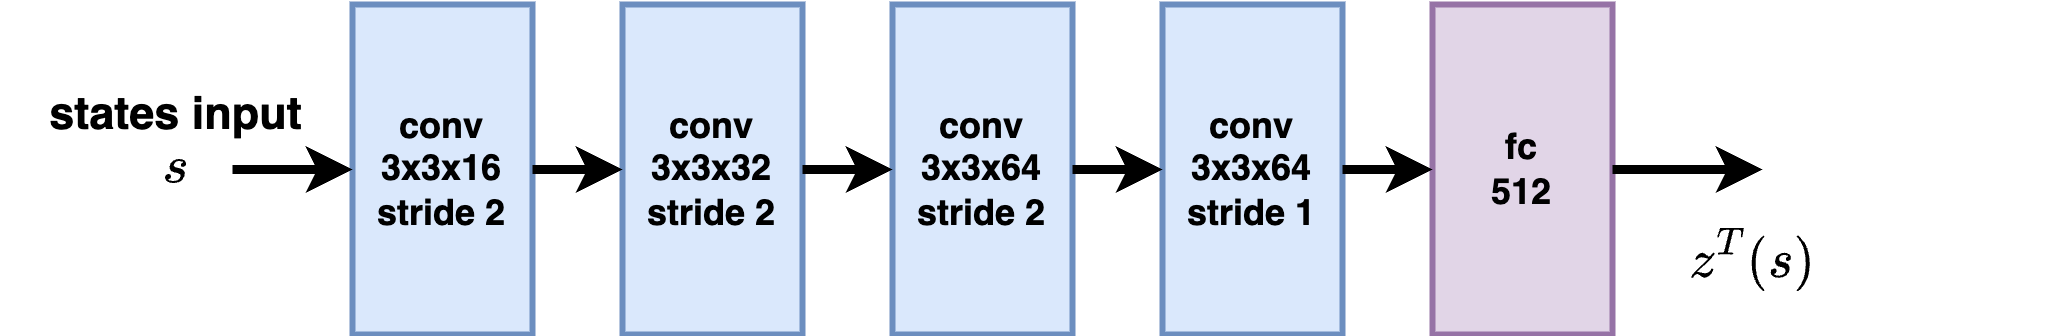
\includegraphics[width=11cm]{fig/diagrams/cnd-target_arch.png}
\caption{The target model architecture.}
\label{img:cnd_target_arch}
\end{figure*}
\begin{figure*}[t!]
\centering
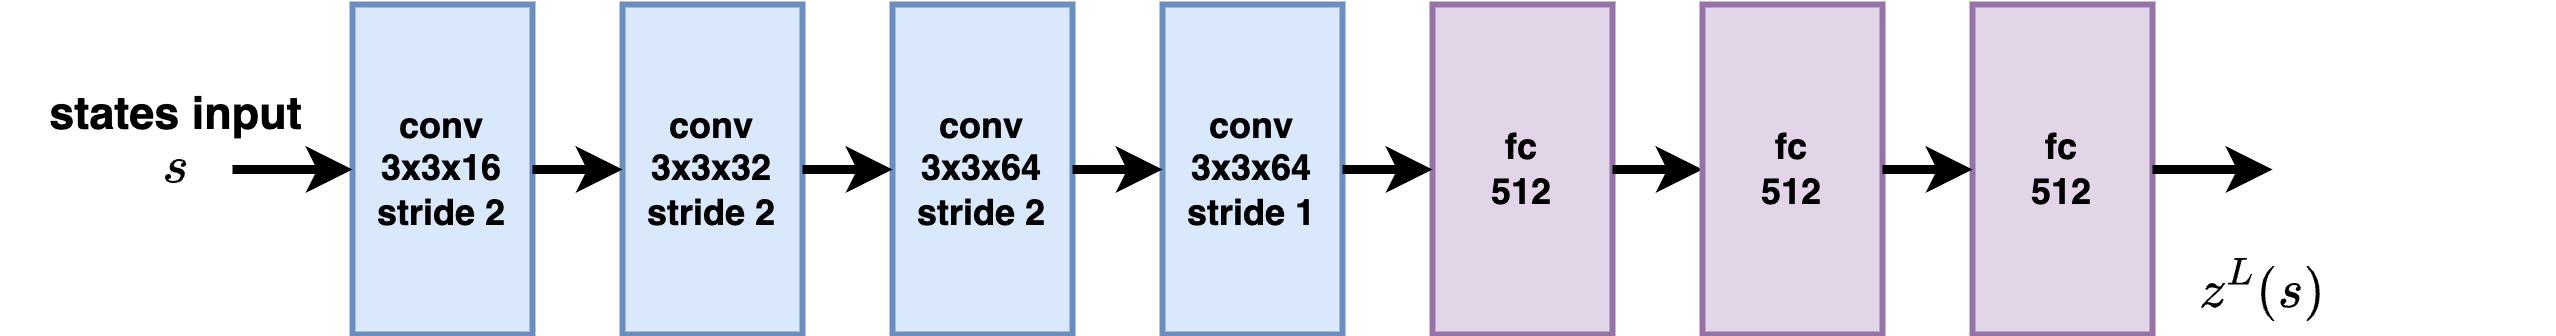
\includegraphics[width=13cm]{fig/diagrams/cnd-learned_arch.png}
\caption{The learning model architecture.}
\label{img:cnd_learned_arch}
\end{figure*}



We followed \citep{burda2018exploration} for setting the hyperparameters, to have more comparable results. We ran 128 parallel environments.
For Atari we used 1M samples for each environment  (total 128M frames), for Procgen we used 0.5M samples for each environment (total 64M frames). 
In Atari experiments we used gray scale downsampled 4 frames stacked observation. 
For Procgen we used 2 frames stacking, and fully RGB colored observation. The intrinsic motivation modules used no frame stacking, a single gray scale image for Atari  environments and a single RGB image for Procgen.
The summary of all environment hyperparameters is in Table \ref{tab:env_hyperparameters}.
The discount factors were set to $\gamma^{\rm ext} = 0.998$ for external reward and $\gamma^{\rm intr} = 0.99$ for intrinsic reward.
We found the importance of intrinsic reward scaling, the best result were achieved for $\eta = 0.5$.
The learning rate for all models was set to 0.0001 with Adam optimizer. Actor and Critic models used ReLU, and motivation models worked best with ELU activation function. We also find the deeper model with 3$\times$3 convolutions works better then standart Atari model using 8$\times$8 or 4$\times$4 convolutions in \citep{mnih2013playing}. We retrained RND models to obtain comparable results and find faster convergence. The summary of PPO agent's hyperparameters is in Table \ref{tab:agent_hyperparameters}.
More hyperparameters and further details of the learning process and the architectures of modules can be found in our source codes.

\begin{table}[thb]
\scriptsize
\centering
\caption{Environment hyperparameters}
    \begin{tabular}{l|ll}
        Hyperparameter & Atari & Procgen  \\ 
        \hline\hline
        Observation downsampling & 96$\times$96 & 64$\times$64 \\
        Frame stacking & 4 & 2 \\
        State shape for PPO & 4$\times$96$\times$96 & 6$\times$64$\times$64 \\
        State shape for IM modules & 1$\times$96$\times$96 & 3$\times$64$\times$64 \\
        Parallel environments count & 128 & 128 \\
        State normalisation & $s/255$ & $s/255$ \\
        Samples per environment & 1M & 0.5M \\
        \hline
    \end{tabular}
    \label{tab:env_hyperparameters}
\end{table}

\begin{table}[thb]
\scriptsize
\centering
\caption{Agent's hyperparameters}
    \begin{tabular}{l|l}
        Hyperparameter & Value \\ 
        \hline\hline
        PPO model learning rate & $0.0001$ \\
        Target model $\Phi^{\rm T}$ learning rate & $0.0001$ \\
        Learned model $\Phi^{\rm L}$ learning rate & $0.0001$ \\
        Discount factor $\gamma^{\rm ext}$ & $0.998$ \\
        Discount factor $\gamma^{\rm intr}$ & $0.99$ \\
        Advantages ext coefficient & $2.0$ \\
        Advantages intr coefficient & $1.0$ \\
        Intrinsic reward scaling & $0.5$ \\
        Rollout length & $128$ \\ 
        Number of optimization epochs & $4$ \\
        Entropy coefficient & $0.001$ \\
        Epsilon clipping & $0.1$ \\
        Gradient norm clipping & $0.5$ \\
        GAE $\lambda$ coefficient & $0.95$ \\
        Optimizer & Adam \\
        Weight initialisation & orthogonal \\
        \hline
    \end{tabular}
    \label{tab:agent_hyperparameters}
\end{table}

\subsection{State preprocessing}
\label{sec:exp2}

The state before entering the motivation module of SND model can undergo preprocessing. We tested three preprocessing methods:
\begin{enumerate}
\item State normalization using the running mean and standard deviation, 
\item Subtraction of the running mean value from the state, 
\item No preprocessing.
\end{enumerate}

We performed two training runs for each preprocessing method in 32M steps on Montezuma's Revenge environment. For testing we used SND-STD model. Table~\ref{tab:res1} demonstrates that the state preprocessing did not have a significant effect on agent's performance (maximum reward achieved), only on the speed of learning. This also agrees with our assumption that operations such as subtraction of the mean or normalization should be able to find the network itself trained using the self-supervised loss function. Therefore it is not necessary for the designer to put them into the learning process explicitly. These conclusions will still need to be confirmed by statistical analysis. RND used mean subtraction and SND-V, SND-STD together with SND-VIC did not use input state preprocessing.

\begin{figure*}[t!]
\centering
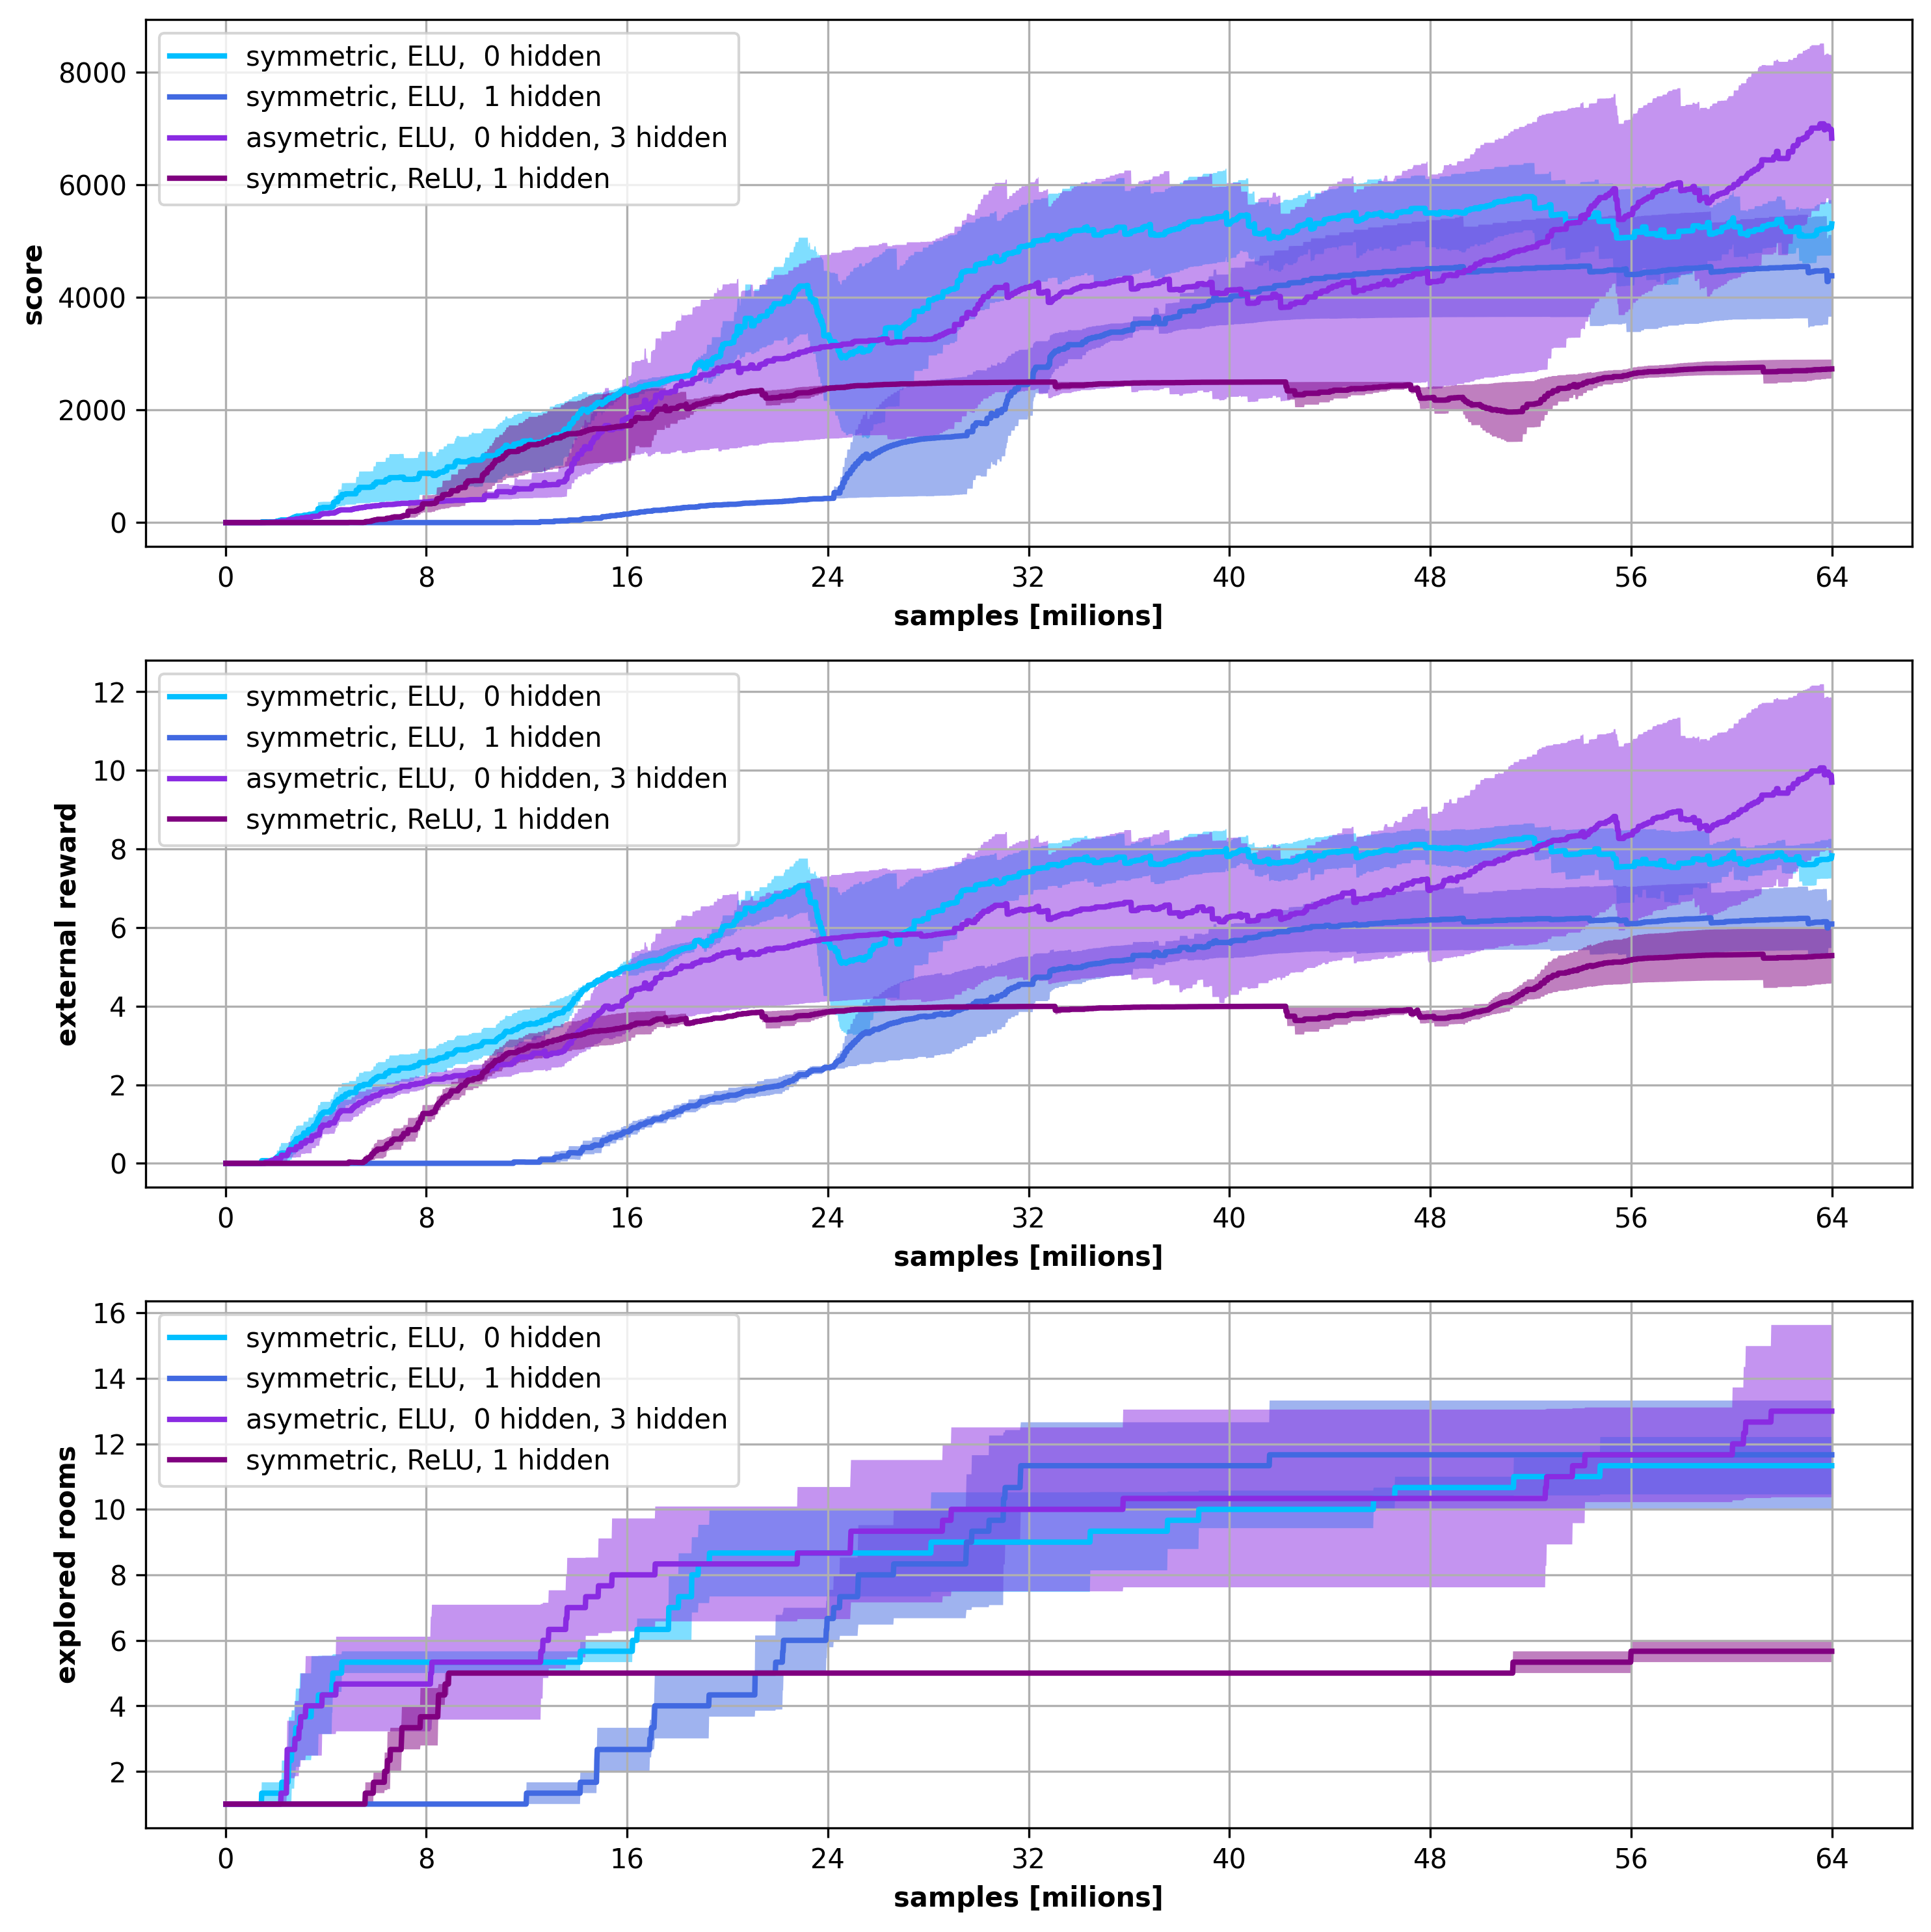
\includegraphics[width=10cm]{fig/results/aux_experiments/cnd_vicreg_architecture.png}
\caption{Agent's performance based on various learned model architectures, evaluated in terms of the overall score, external reward obtained and the number of rooms explored.}
\label{img:result_cnd_learned_arch}
\end{figure*}

\begin{table}[thb]
\scriptsize
\centering
\caption{Average cumulative reward (with standard deviation) per episode for all 3 preprocessing methods and maximal reward achieved by the agents.}
\begin{tabular}{l|ll}
Method & Average reward & Max. reward \\
\hline\hline
normalization    & 3.60 $\pm$ 0.14 & 7 \\ 
mean subtraction & 4.13 $\pm$ 0.12 & 7 \\
none & 2.31 $\pm$ 0.20 & 7 \\
\hline
\end{tabular}
\label{tab:res1}
\end{table}

\subsection{Results}

We processed several quick experiments on Montezuma's Revenge to explore an optimal setup.
First we have to test the optimal architecture of $\Phi^{\rm T}$ and $\Phi^{\rm L}$ models. 
We experimented with 4 architectures: 
\begin{enumerate}
    \item identical models, one fully connected output layer, ELU activations
    \item identical models, two fully connected layers, ELU activations
    \item identical models, one fully connected layer, ReLU activations
    \item asymmetric models, three fully connected layers for $\Phi^{\rm L}$, none for $\Phi^{\rm T}$, ELU activations fixed to fully connected convention
\end{enumerate}
Results of different model architectures are in Figure~\ref{img:result_cnd_learned_arch}. The best result was achieved for the asymmetric architecture.

Next, we tested the effect of different augmentations. We considered three scenarios: 
\begin{enumerate}
    \item uniform noise, $\langle -0.2, 0.2 \rangle$
    \item uniform noise, random tiles masking (tiles with sizes 1, 2, 4, 8, 12, 16)
    \item uniform noise,  random tiles masking, random convolution filter apply
\end{enumerate}

\begin{figure*}[t!]
\centering
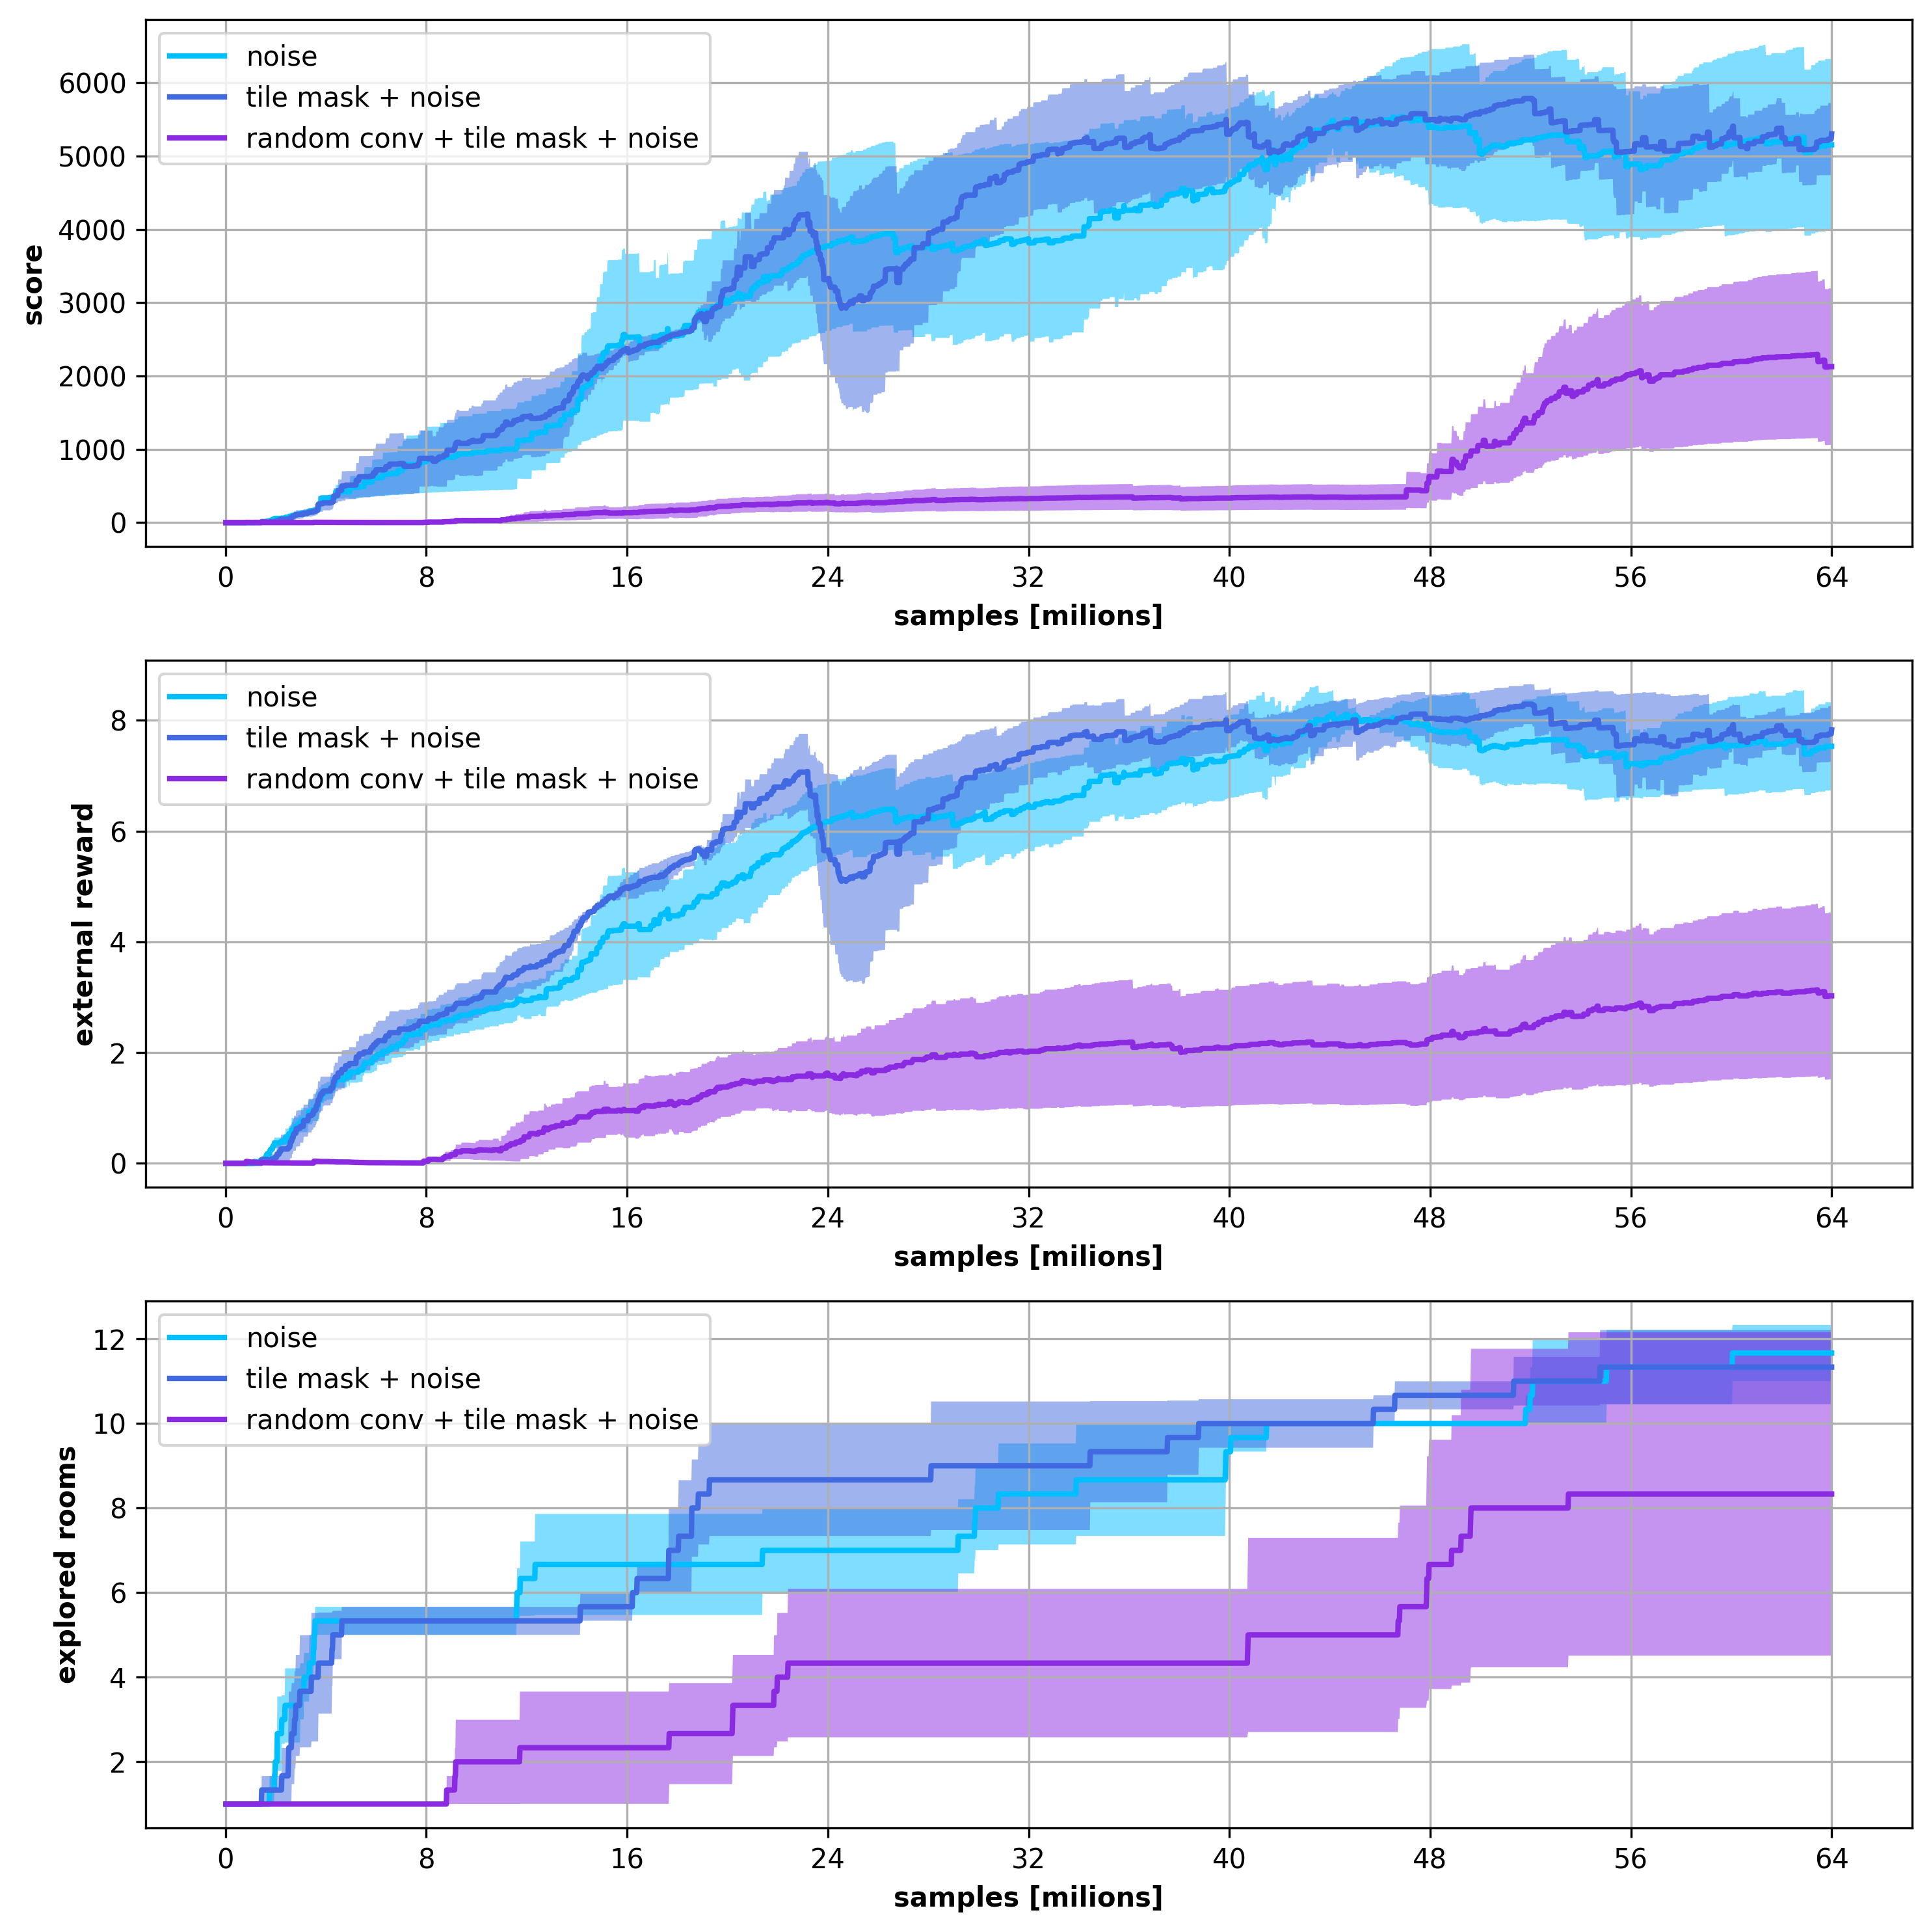
\includegraphics[width=10cm]{fig/results/aux_experiments/cnd_vicreg_augmentations.png}
\caption{Agent performance for different state augmentations, evaluated in terms of the overall score, external reward obtained and the number of rooms explored.}
\label{img:result_cnd_aug}
\end{figure*}

Noise augmentation is commonly used in supervised image training. Tile masking
forces the model to reconstruct non-complete information. Random convolution filter
helps the model to learn to focus on informative features, not on texture colors. The results of different state augmentations are in Figure~\ref{img:result_cnd_aug}, revealing that the third scenario worked best. We hypothesise that it is caused by shallow target model, which is not able to learn sufficient transformation invariants. The models using noise or tile masking performed in a similar way.


\begin{figure*}[t!]
\centering
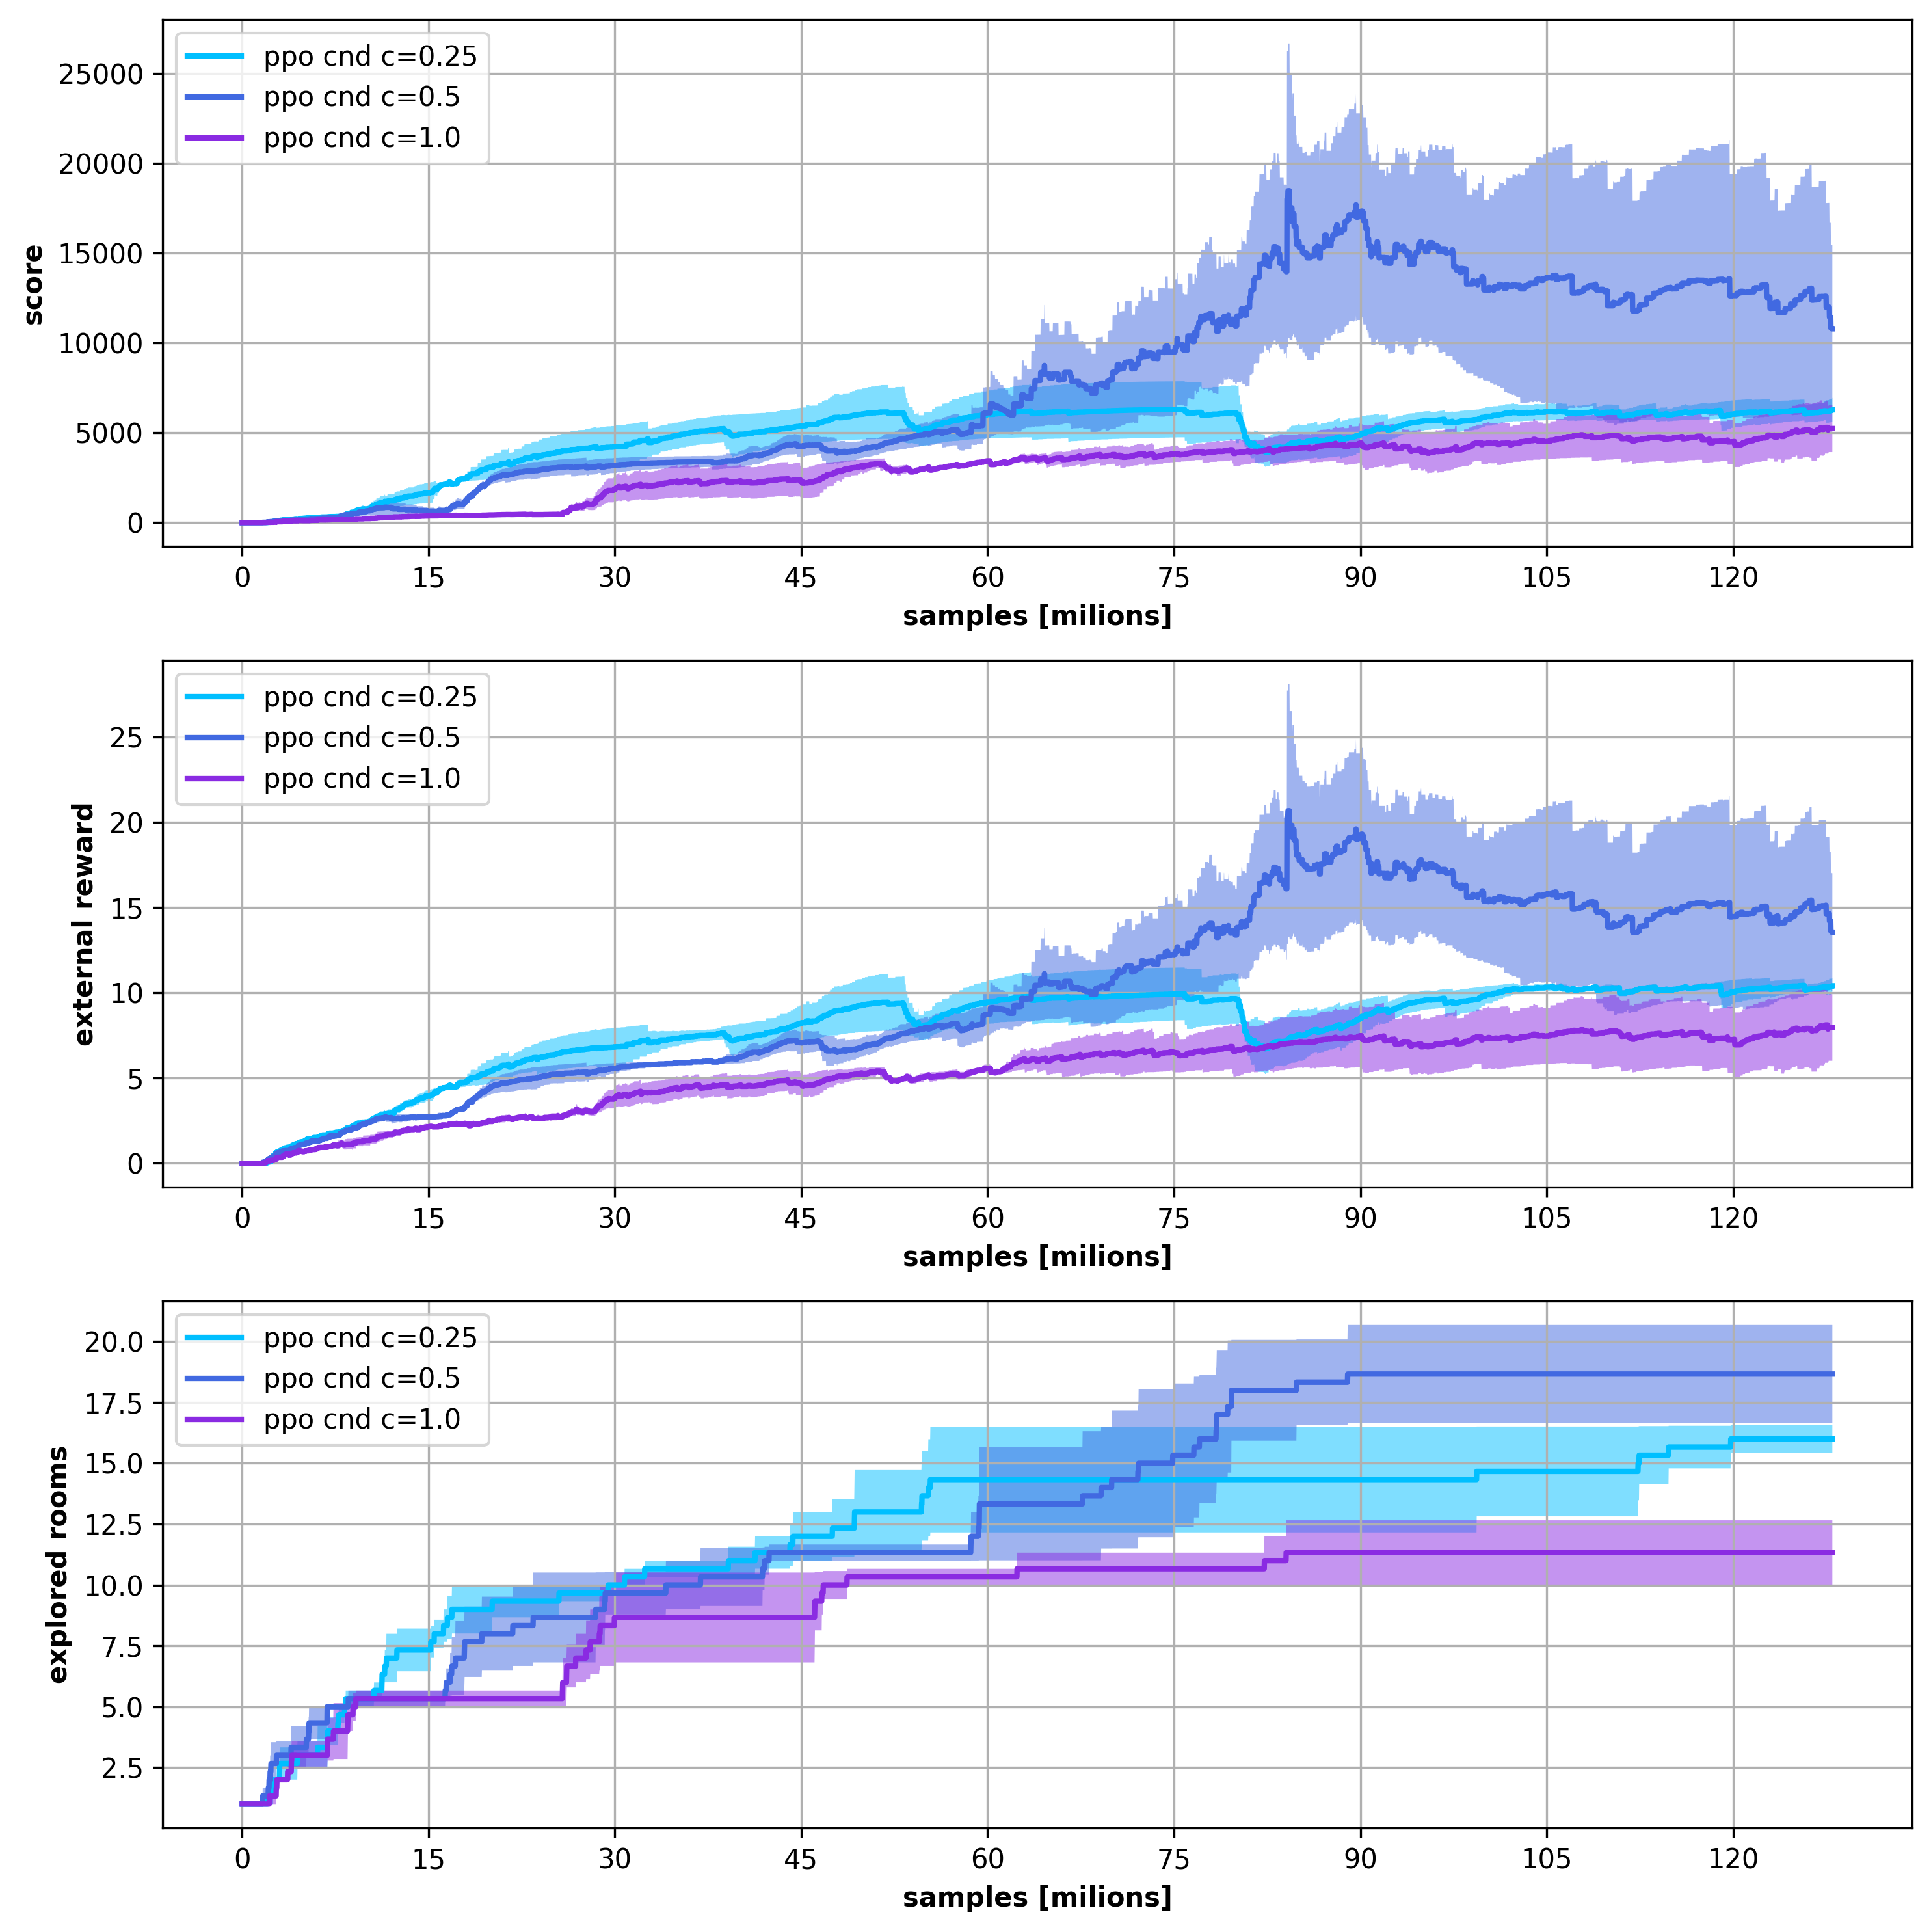
\includegraphics[width=10cm]{fig/results/aux_experiments/cnd_scaling.png}
\caption{Agent's performance for different intrinsic reward scaling methods, evaluated in terms of the overall score, external reward obtained and the number of rooms explored.}
\label{img:result_cnd_scaling}
\end{figure*}

\begin{figure}[t!]
  \centering
  \begin{subfigure}[b]{0.32\textwidth}
    \centering
    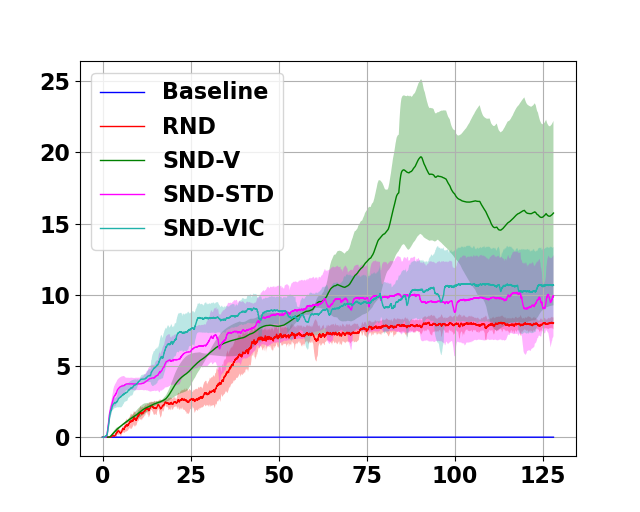
\includegraphics[width=4.1cm]{fig/results/montezuma.png}
    \caption{Montezuma's Revenge}
    \label{fig:res2a}
  \end{subfigure}
  \begin{subfigure}[b]{0.32\textwidth}
    \centering
    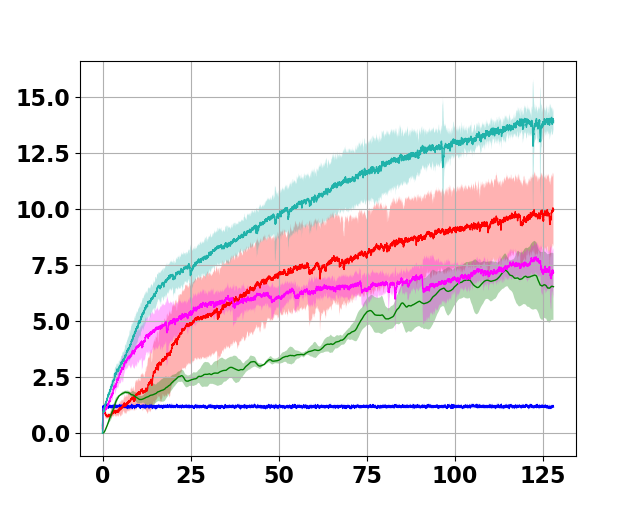
\includegraphics[width=4.1cm]{fig/results/gravitar.png}
    \caption{Gravitar}
    \label{fig:res2b}
  \end{subfigure}  
  \begin{subfigure}[b]{0.32\textwidth}
    \centering
    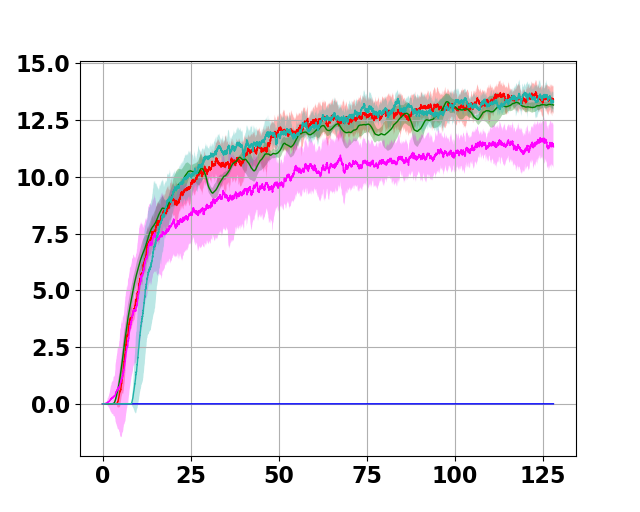
\includegraphics[width=4.1cm]{fig/results/venture.png}
    \caption{Venture}
    \label{fig:res2c}
  \end{subfigure}
  \begin{subfigure}[b]{0.32\textwidth}
    \centering
    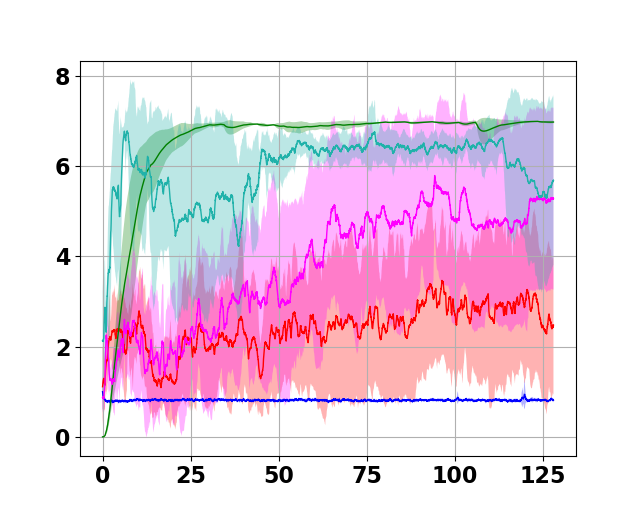
\includegraphics[width=4.1cm]{fig/results/private_eye.png}
    \caption{Private Eye}
    \label{fig:res2d}
  \end{subfigure} 
  \begin{subfigure}[b]{0.32\textwidth}
    \centering
    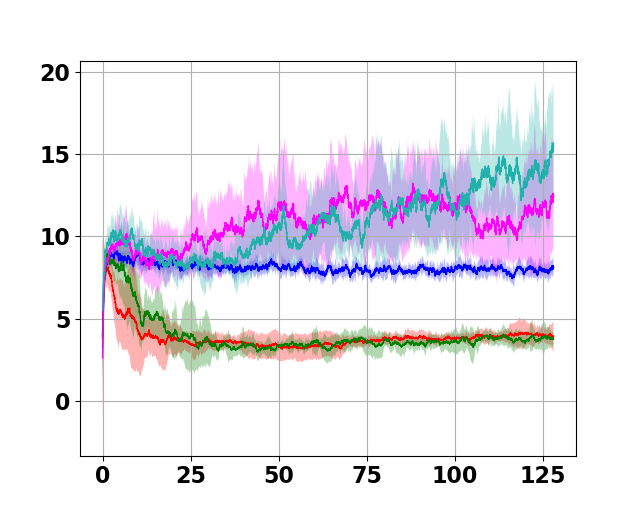
\includegraphics[width=4.1cm]{fig/results/solaris.png}
    \caption{Solaris}
    \label{fig:res2f}
  \end{subfigure}
    \begin{subfigure}[b]{0.32\textwidth}
    \centering
    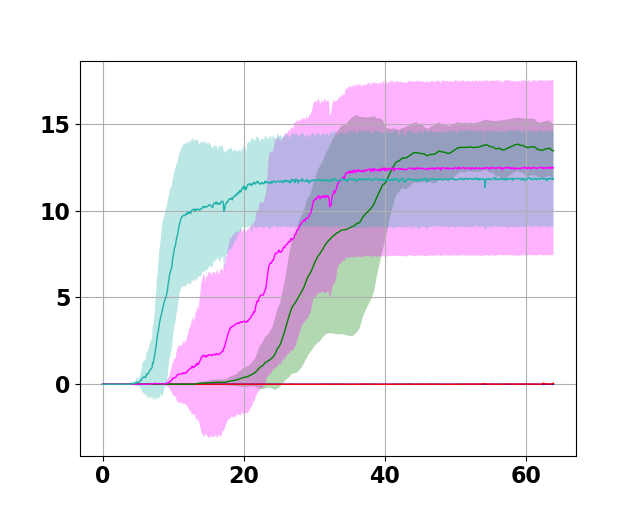
\includegraphics[width=4.1cm]{fig/results/caveflyer.png}
    \caption{Caveflyer}
    \label{fig:res2g}
  \end{subfigure}
    \begin{subfigure}[b]{0.32\textwidth}
    \centering
    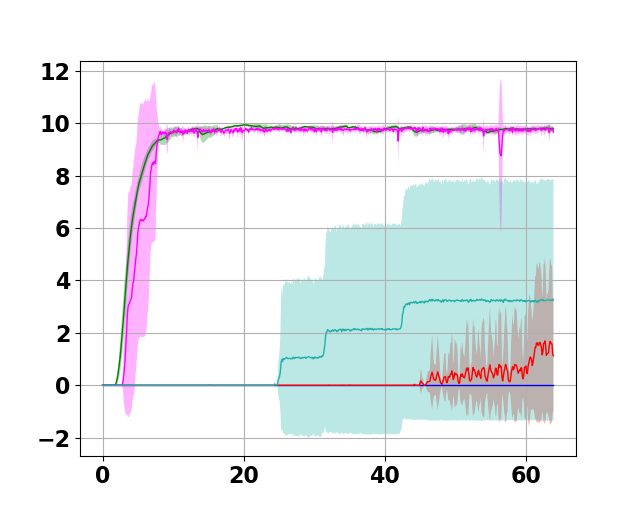
\includegraphics[width=4.1cm]{fig/results/coinrun.png}
    \caption{Coinrun}
    \label{fig:res2h}
  \end{subfigure}
    \begin{subfigure}[b]{0.32\textwidth}
    \centering
    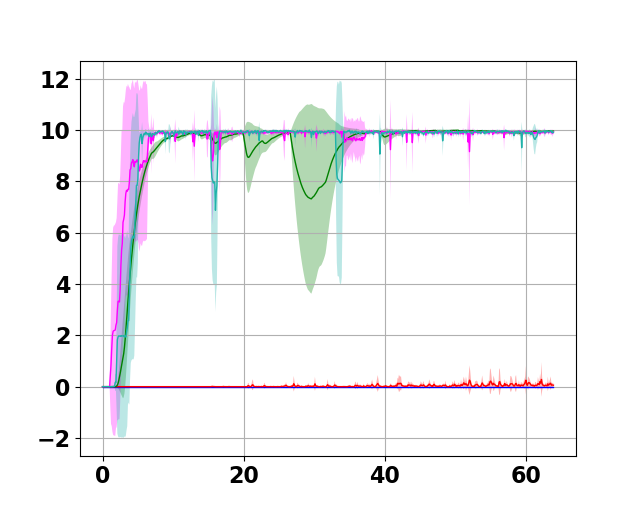
\includegraphics[width=4.1cm]{fig/results/jumper.png}
    \caption{Jumper}
    \label{fig:res2i}
  \end{subfigure}
    \begin{subfigure}[b]{0.32\textwidth}
    \centering
    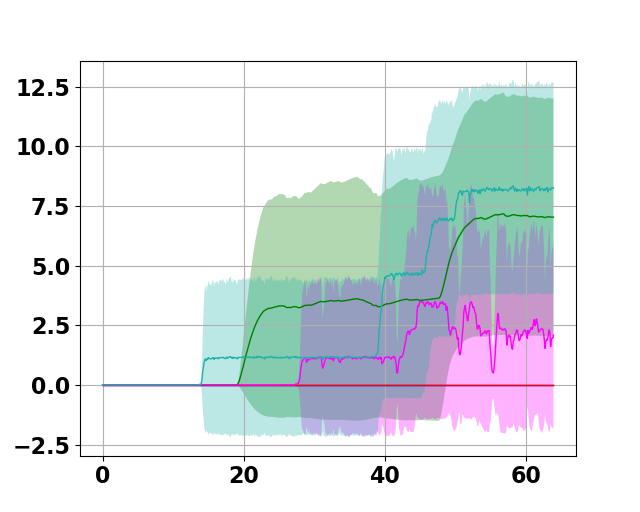
\includegraphics[width=4.1cm]{fig/results/climber.png}
    \caption{Climber}
    \label{fig:res2j}
  \end{subfigure}
\caption{The cumulative external reward per episode (with the standard deviation) received by the agent from the tested environment. We omitted the graph for the Pitfall environment, where no algorithm was successful and all achieved zero reward. The horizontal axis shows the number of steps in millions, the vertical axis refers the external reward.}
\label{fig:result}
\end{figure}

\begin{table}[thb]
\scriptsize
\centering
\caption{Average cumulative external reward per episode for tested models. The best model for each environment is shown in bold face.}
\begin{tabular}{l|cccccc}
\hline
 & Baseline & RND & SND-V & SND-STD & SND-VIC \\
\hline\hline
Montezuma & 0.00 $\pm$ 0.00 & 5.33 $\pm$ 0.23 & \textbf{10.59 $\pm$ 1.99} & 7.76 $\pm$ 1.73 & 8.45 $\pm$ 1.12 \\
Gravitar & 1.19 $\pm$ 0.00 & 6.63 $\pm$ 1.55 & 4.38 $\pm$ 0.46 & 5.89 $\pm$ 0.43 &\textbf{ 10.05 $\pm$ 0.66} \\
Venture & 0.00 $\pm$ 0.00 & 11.18 $\pm$ 0.42 & 10.95 $\pm$ 0.14 & 9.54 $\pm$ 0.90 & \textbf{11.36 $\pm$ 0.37} \\ 
Private Eye & 0.81 $\pm$ 0.01 & 2.41 $\pm$ 0.95 & \textbf{6.59 $\pm$ 0.14} & 3.79 $\pm$ 1.24 & 5.93 $\pm$ 0.47  \\ 
Pitfall & 0.00 $\pm$ 0.00 & 0.00 $\pm$ 0.00 & 0.00 $\pm$ 0.00 & 0.00 $\pm$ 0.00 & 0.00 $\pm$ 0.00 \\ 
Solaris & 8.08 $\pm$ 0.15 & 3.84 $\pm$ 0.25 & 3.96 $\pm$ 0.41 & \textbf{11.61 $\pm$ 1.12} & 10.85 $\pm$ 1.20  \\
Caveflyer & 0.00 $\pm$ 0.00 & 0.00 $\pm$ 0.00 & 7.28 $\pm$ 1.62 & 10.86 $\pm$ 4.37 & \textbf{11.14 $\pm$ 2.35} \\
Coinrun & 0.00 $\pm$ 0.00 & 0.25 $\pm$ 0.50 & \textbf{9.40 $\pm$ 0.05} & 9.40 $\pm$ 0.07 & 2.55 $\pm$ 3.63  \\
Jumper & 0.00 $\pm$ 0.00 & 0.03 $\pm$ 0.02 & 9.22 $\pm$ 0.21 & 9.76 $\pm$ 0.04 & \textbf{9.76 $\pm$ 0.03}\\
Climber & 0.00 $\pm$ 0.00 & 0.00 $\pm$ 0.00 & 3.32 $\pm$ 3.04 & 1.48 $\pm$ 2.40 & \textbf{4.93 $\pm$ 2.88} \\
\hline
\end{tabular}
\label{tab:res2}
\end{table}

\begin{table}[thb]
\scriptsize
\centering
\caption{Average maximal score reached by tested models on Atari environments. The best model for each environment is shown in bold face.}
\begin{tabular}{l|cccccc}
\hline
 & Baseline & RND & SND-V & SND-STD & SND-VIC \\
\hline\hline
Montezuma & 400 & 6689 & \textbf{21565} & 7212 & 7838 \\
Gravitar & 2611 & 5600 & 2741 & 4643 & \textbf{6712} \\
Venture & 22 & 2167 & 1787 & 2138 & \textbf{2188}  \\ 
Private Eye & 14870 & 14996 & 4213 & 15089 & \textbf{17313} \\ 
Pitfall & 0 & 0 & 0 & 0 & 0 \\ 
Solaris & 12344 & 10667 & 11582 & \textbf{12460} & 11865 \\ 
\hline
\end{tabular}
\label{tab:res3}
\end{table}

Finally, we tested intrinsic reward scaling. Low value can lead to stacking the agent into non-exploring policy. High value can prevent the agent from collecting extrinsic rewards, or make it too sensitive to small unimportant changes, both causing instability. We tested three values 0.25, 0.5 and 1.0. Figure~\ref{img:result_cnd_scaling} shows that the best score is achieved with 0.5 reward scaling value. However, some environments provide better results after fine-tuning to 0.25.

Figure~\ref{fig:result} captures the cumulative external reward per episode and the standard deviation of the tested models in 9 different environments. In Table~\ref{tab:res2}, these indicators are then averaged over the number of episodes. Table~\ref{tab:res3} shows the maximum achieved score for Atari environments, which is often used for model comparison (although we would like to emphasize that the agent never receives this score as a reward and therefore it is not its goal to maximize it).
Of the tested environments, Pitfall game exceeded the capabilities of all tested algorithms, since none of them achieved a single reward point. In the remaining 9 environments, the best results were achieved with the models based on SND motivation, while in 8 cases it was with a significant lead over the existing algorithms (in Venture environment the results were almost the same as those of the RND model). When evaluating the score, the SND models achieved the highest score in 5 Atari environments (with an exception of the already mentioned Pitfall) and in 3 cases (Montezuma's Revenge, Gravitar, Private Eye) it was significantly higher than the compared models.

\subsection{Analysis of results}

\begin{figure}[thb]
  \begin{subfigure}{0.5\textwidth}
    \centering
    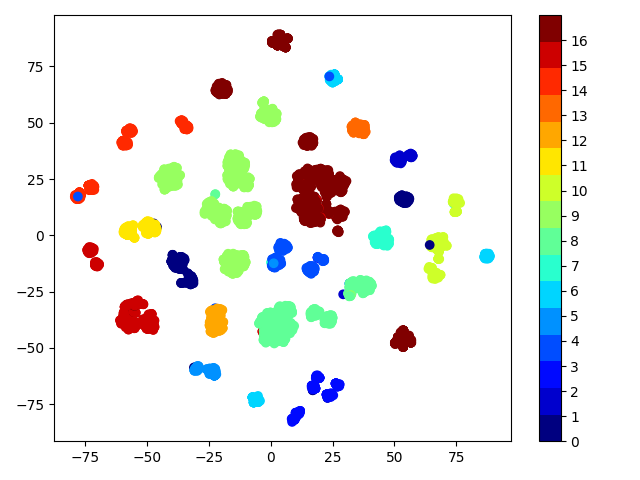
\includegraphics[width=7cm]{fig/images/cnd_random.png}
    \caption{Random target model}
    \label{fig:target_features_random}
  \end{subfigure}
  \begin{subfigure}{0.5\textwidth}
    \centering
    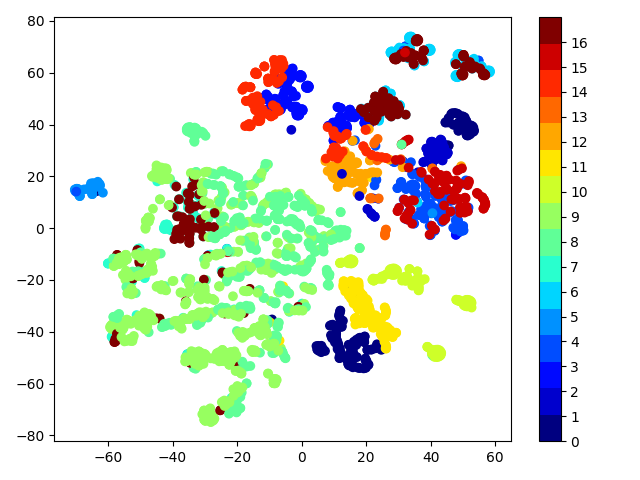
\includegraphics[width=7cm]{fig/images/cnd_trained.png}
    \caption{Trained target model}
    \label{fig:trained_features_random}
  \end{subfigure}  
\caption{The t-SNE projected feature representations of the target model in Montezuma's Revenge task. The colors correspond to different rooms.}
\label{fig:cnd_feature_space}
\end{figure}

\begin{figure}[t!]
  \centering
  \begin{subfigure}[b]{0.3\textwidth}
    \centering
    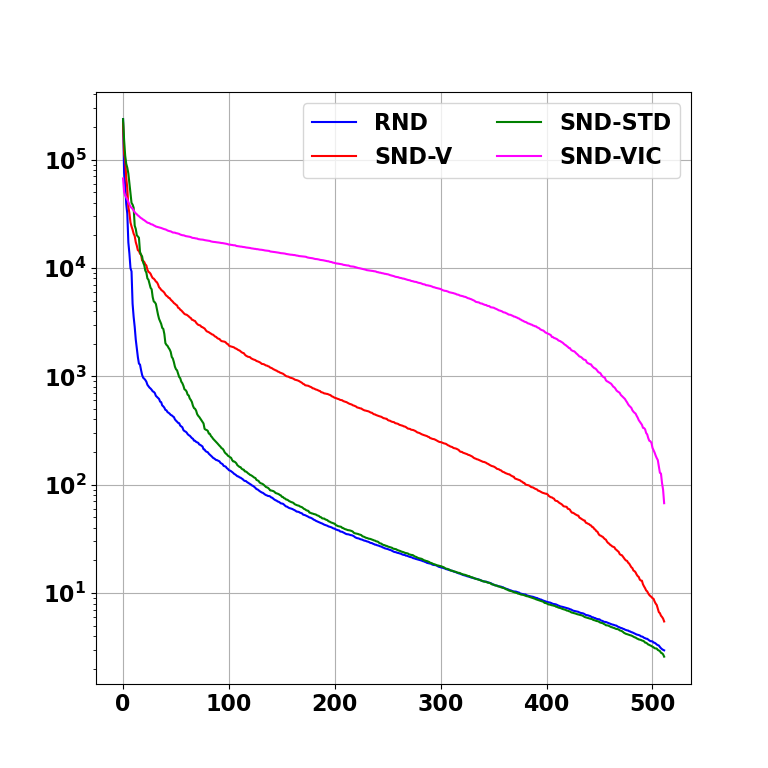
\includegraphics[width=4cm]{fig/analysis/anal_montezuma.png}
    \caption{Montezuma's Revenge}
    \label{fig:analysis2a}
  \end{subfigure}
  \begin{subfigure}[b]{0.3\textwidth}
    \centering
    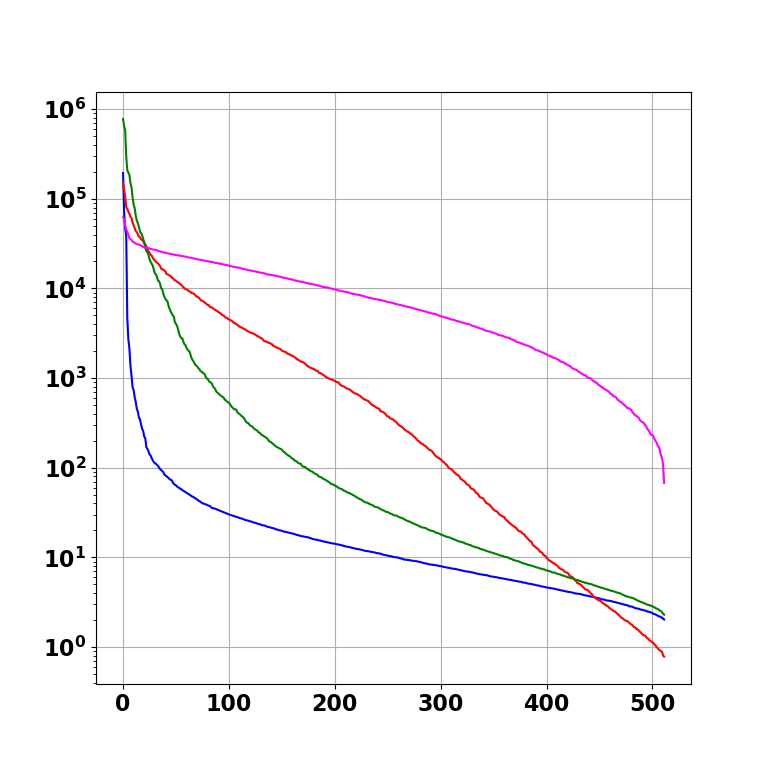
\includegraphics[width=4cm]{fig/analysis/anal_gravitar.png}
    \caption{Gravitar}
    \label{fig:analysis2b}
  \end{subfigure}  
  \begin{subfigure}[b]{0.3\textwidth}
    \centering
    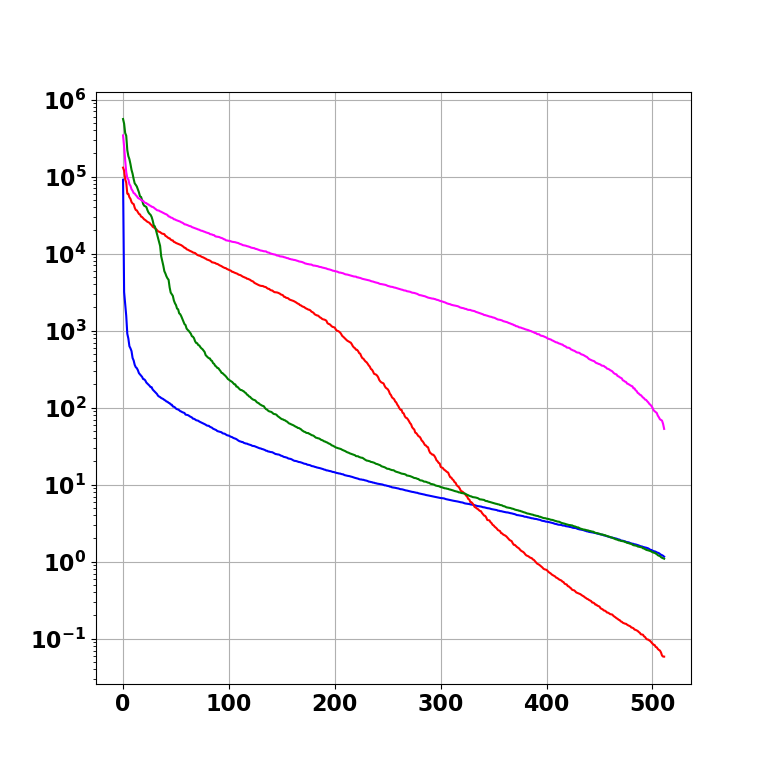
\includegraphics[width=4cm]{fig/analysis/anal_venture.png}
    \caption{Venture}
    \label{fig:analysis2c}
  \end{subfigure}
  \begin{subfigure}[b]{0.3\textwidth}
    \centering
    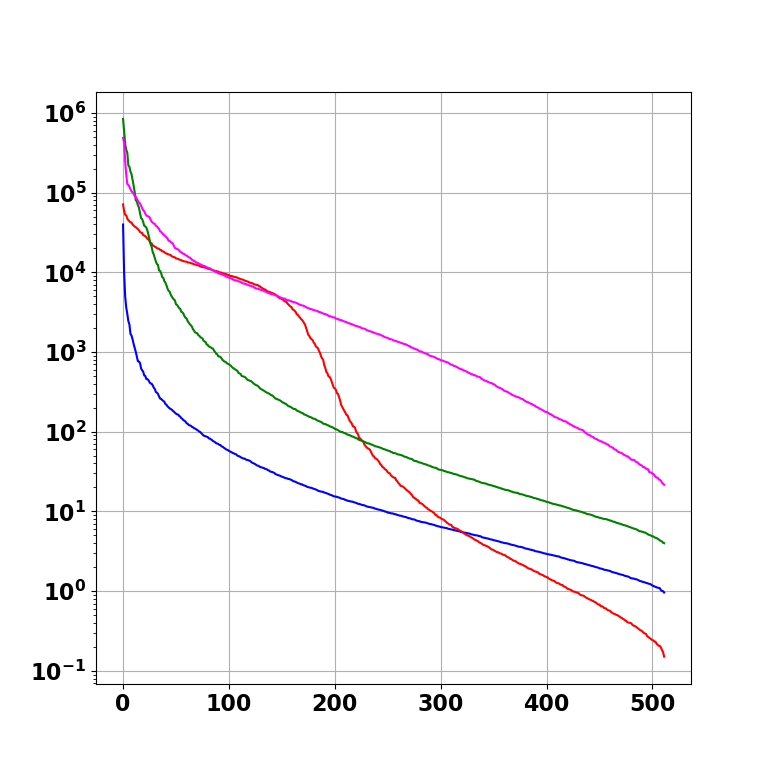
\includegraphics[width=4cm]{fig/analysis/anal_private_eye.png}
    \caption{Private Eye}
    \label{fig:analysis2d}
  \end{subfigure} 
  \begin{subfigure}[b]{0.3\textwidth}
    \centering
    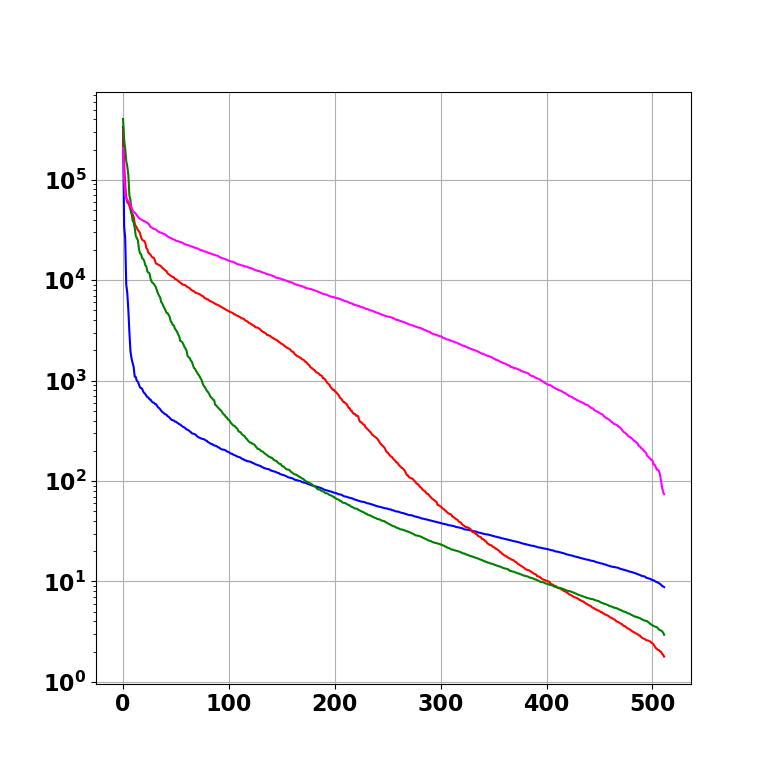
\includegraphics[width=4cm]{fig/analysis/anal_solaris.png}
    \caption{Solaris}
    \label{fig:analysis2e}   
  \end{subfigure}
    \begin{subfigure}[b]{0.3\textwidth}
    \centering
    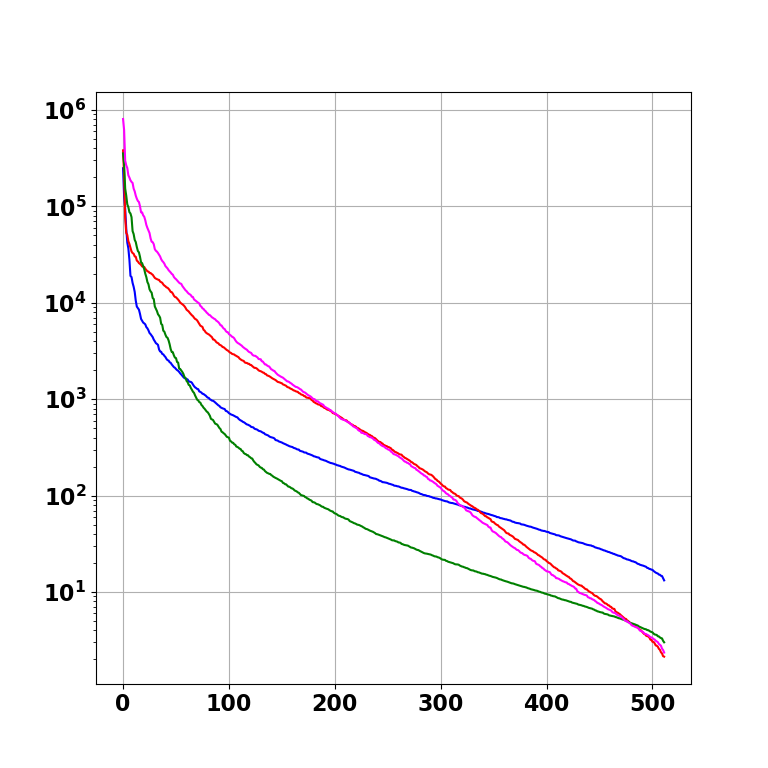
\includegraphics[width=4cm]{fig/analysis/anal_caveflyer.png}
    \caption{Caveflyer}
    \label{fig:analysis2f}
  \end{subfigure}
  \begin{subfigure}[b]{0.3\textwidth}
    \centering
    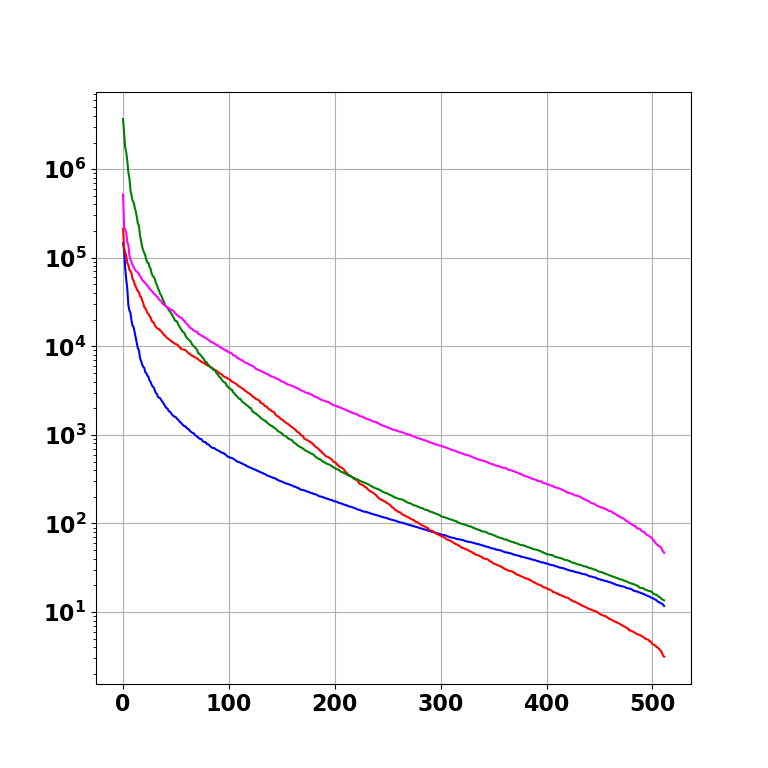
\includegraphics[width=4cm]{fig/analysis/anal_coinrun.png}
    \caption{Coinrun}
    \label{fig:analysis2g}
  \end{subfigure}
  \begin{subfigure}[b]{0.3\textwidth}
    \centering
    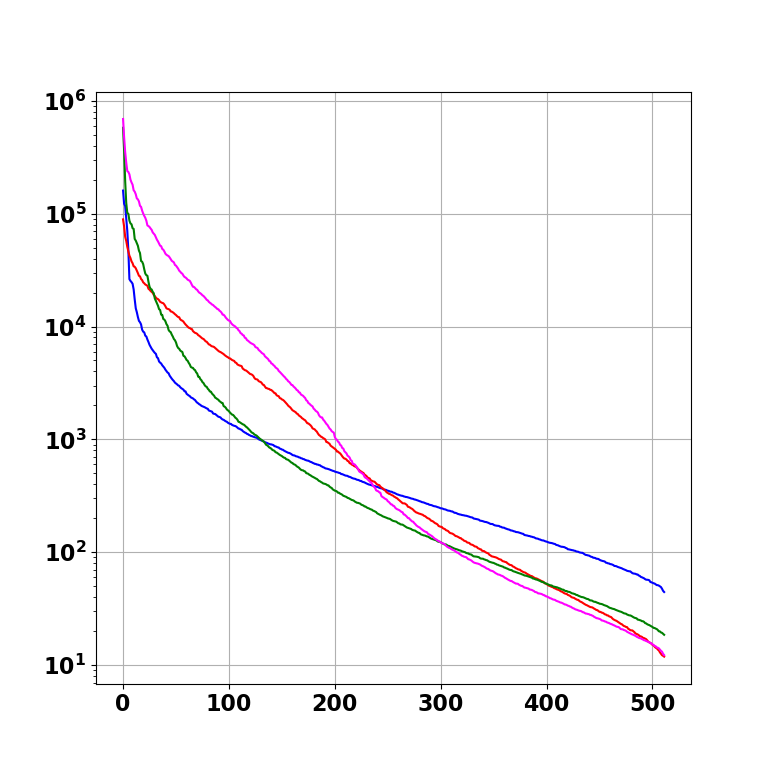
\includegraphics[width=4cm]{fig/analysis/anal_jumper.png}
    \caption{Jumper}
    \label{fig:analysis2h}
  \end{subfigure}
    \begin{subfigure}[b]{0.3\textwidth}
    \centering
    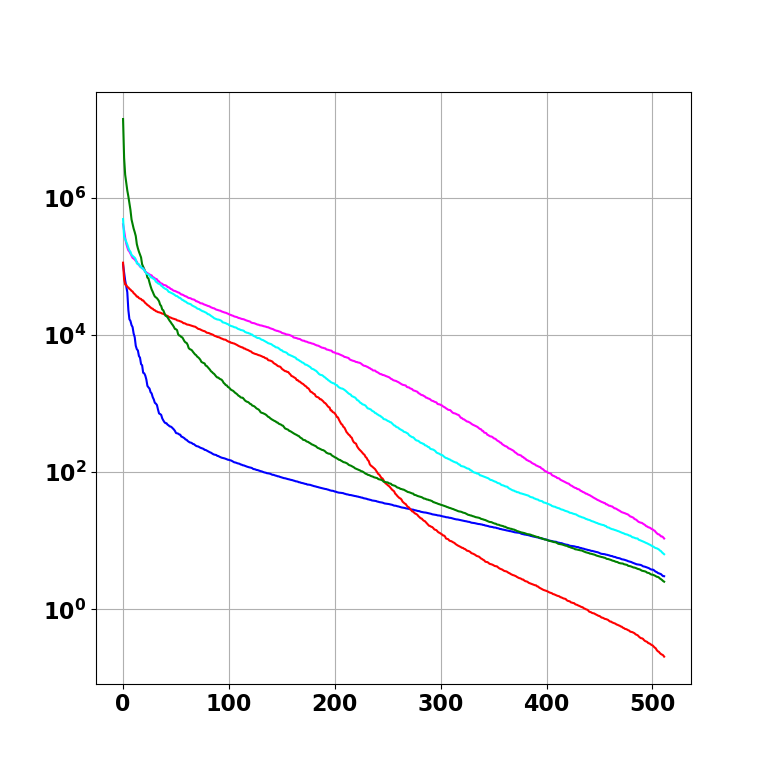
\includegraphics[width=4cm]{fig/analysis/anal_climber.png}
    \caption{Climber}
    \label{fig:analysis2i}
  \end{subfigure}
\caption{Descendingly ordered eigenvalues of the linear envelope obtained using the PCA method, which show the stretching of the feature space in individual dimensions. 
The horizontal axis shows the indices of eigenvalues, the vertical axis denotes the magnitude of eigenvalue in logarithmic scale.
Based on these data, we tried to find out if there is a connection between the shape of the feature space and the performance of the given model. The graph for Pitfall was omitted, since it looked very similar to Private Eye. }
\label{fig:cnd_analysis}
\end{figure}

\iffalse

\begin{table}[t!]
\scriptsize
\centering
\caption{Description of the target model feature space created by four selected methods. For the evaluation, we used the following parameters: mean value and standard deviation of the $L_{2}$-norm of features, 25th, 50th, 75th and 95th percentiles of eigenvalues of a linear envelop to obtain a rough representation of stretching of the feature space in individual dimensions. To this, we add the maximum achieved external reward ($\max{r_{\rm ext}}$), so that it is possible to search for a connection between the parameters of the feature space and the performance of the method.}
\begin{tabular}{l|l|cccccc}
\hline
 Environment & Method & $\max({r_{\rm ext}})$ & $L_2$-norm & $Q_{25}$ & $Q_{50}$ & $Q_{75}$ & $Q_{95}$ \\
\hline\hline
\multirow{4}{*}{Montezuma}
& \multicolumn{1}{l|}{RND} & \multicolumn{1}{c}{9} & \multicolumn{1}{c}{1.93 $\pm$ 1.15} & \multicolumn{1}{c}{9} & \multicolumn{1}{c}{24} & \multicolumn{1}{c}{89} & \multicolumn{1}{c}{778} \\
& \multicolumn{1}{l|}{SND-STD} & \multicolumn{1}{c}{16} & \multicolumn{1}{c}{4.85 $\pm$ 2.45} & \multicolumn{1}{c}{9} & \multicolumn{1}{c}{26} & \multicolumn{1}{c}{109} & \multicolumn{1}{c}{6835} \\
& \multicolumn{1}{l|}{SND-VIC} & \multicolumn{1}{c}{17} & \multicolumn{1}{c}{6.22 $\pm$ 2.99} & \multicolumn{1}{c}{3066} & \multicolumn{1}{c}{8429} & \multicolumn{1}{c}{14858} & \multicolumn{1}{c}{25634} \\
& \multicolumn{1}{l|}{SND-V} & \multicolumn{1}{c}{34} & \multicolumn{1}{c}{6.41 $\pm$ 3.96} & \multicolumn{1}{c}{98} & \multicolumn{1}{c}{378} & \multicolumn{1}{c}{1367} & \multicolumn{1}{c}{8944} \\
\hline%\hline
\multirow{4}{*}{Gravitar}
& \multicolumn{1}{l|}{SND-V} & \multicolumn{1}{c}{9} & \multicolumn{1}{c}{11.94 $\pm$ 3.81} & \multicolumn{1}{c}{16} & \multicolumn{1}{c}{341} & \multicolumn{1}{c}{2919} & \multicolumn{1}{c}{24291} \\
& \multicolumn{1}{l|}{SND-STD} & \multicolumn{1}{c}{15} & \multicolumn{1}{c}{11.66 $\pm$ 2.82} & \multicolumn{1}{c}{8} & \multicolumn{1}{c}{30} & \multicolumn{1}{c}{250} & \multicolumn{1}{c}{20402} \\
& \multicolumn{1}{l|}{RND} & \multicolumn{1}{c}{20} & \multicolumn{1}{c}{1.12 $\pm$ 0.81} & \multicolumn{1}{c}{5} & \multicolumn{1}{c}{10} & \multicolumn{1}{c}{24} & \multicolumn{1}{c}{139} \\
& \multicolumn{1}{l|}{SND-VIC} & \multicolumn{1}{c}{21} & \multicolumn{1}{c}{7.26 $\pm$ 3.01} & \multicolumn{1}{c}{2263} & \multicolumn{1}{c}{6837} & \multicolumn{1}{c}{15173} & \multicolumn{1}{c}{27908} \\
\hline%\hline
\multirow{4}{*}{Private Eye}
& \multicolumn{1}{l|}{SND-V} & \multicolumn{1}{c}{7} & \multicolumn{1}{c}{15.47 $\pm$ 6.50} & \multicolumn{1}{c}{2} & \multicolumn{1}{c}{27} & \multicolumn{1}{c}{6801} & \multicolumn{1}{c}{23823} \\
& \multicolumn{1}{l|}{RND} & \multicolumn{1}{c}{9} & \multicolumn{1}{c}{1.40 $\pm$ 0.65} & \multicolumn{1}{c}{3} & \multicolumn{1}{c}{9} & \multicolumn{1}{c}{37} & \multicolumn{1}{c}{410} \\ 
& \multicolumn{1}{l|}{SND-STD} & \multicolumn{1}{c}{9} & \multicolumn{1}{c}{8.03 $\pm$ 4.46} & \multicolumn{1}{c}{15} & \multicolumn{1}{c}{54} & \multicolumn{1}{c}{371} & \multicolumn{1}{c}{24025} \\
& \multicolumn{1}{l|}{SND-VIC} & \multicolumn{1}{c}{10} & \multicolumn{1}{c}{4.29 $\pm$ 3.56} & \multicolumn{1}{c}{232} & \multicolumn{1}{c}{1401} & \multicolumn{1}{c}{6197} & \multicolumn{1}{c}{47342} \\
\hline%\hline
\multirow{4}{*}{Pitfall}
& \multicolumn{1}{l|}{RND} & \multicolumn{1}{c}{0} & \multicolumn{1}{c}{1.31 $\pm$ 0.39} & \multicolumn{1}{c}{3} & \multicolumn{1}{c}{10} & \multicolumn{1}{c}{47} & \multicolumn{1}{c}{410} \\
& \multicolumn{1}{l|}{SND-V} & \multicolumn{1}{c}{0} & \multicolumn{1}{c}{2.81 $\pm$ 1.43} & \multicolumn{1}{c}{2} & \multicolumn{1}{c}{124} & \multicolumn{1}{c}{7358} & \multicolumn{1}{c}{27402} \\
& \multicolumn{1}{l|}{SND-STD} & \multicolumn{1}{c}{0} & \multicolumn{1}{c}{10.64 $\pm$ 2.81} & \multicolumn{1}{c}{8} & \multicolumn{1}{c}{32} & \multicolumn{1}{c}{319} & \multicolumn{1}{c}{39904} \\
& \multicolumn{1}{l|}{SND-VIC} & \multicolumn{1}{c}{0} & \multicolumn{1}{c}{5.62 $\pm$ 1.79} & \multicolumn{1}{c}{153} & \multicolumn{1}{c}{1542} & \multicolumn{1}{c}{9827} & \multicolumn{1}{c}{44126} \\
\hline%\hline
\multirow{4}{*}{Venture}
& \multicolumn{1}{l|}{SND-V} & \multicolumn{1}{c}{14} & \multicolumn{1}{c}{3.67 $\pm$ 3.07} & \multicolumn{1}{c}{1} & \multicolumn{1}{c}{130} & \multicolumn{1}{c}{3921} & \multicolumn{1}{c}{24443} \\
& \multicolumn{1}{l|}{RND} & \multicolumn{1}{c}{18} & \multicolumn{1}{c}{0.68 $\pm$ 0.80} & \multicolumn{1}{c}{4} & \multicolumn{1}{c}{9} & \multicolumn{1}{c}{30} & \multicolumn{1}{c}{188} \\ 
& \multicolumn{1}{l|}{SND-STD} & \multicolumn{1}{c}{18} & \multicolumn{1}{c}{4.50 $\pm$ 3.79} & \multicolumn{1}{c}{4} & \multicolumn{1}{c}{15} & \multicolumn{1}{c}{115} & \multicolumn{1}{c}{32272} \\
& \multicolumn{1}{l|}{SND-VIC} & \multicolumn{1}{c}{18} & \multicolumn{1}{c}{4.91 $\pm$ 3.89} & \multicolumn{1}{c}{1006} & \multicolumn{1}{c}{3644} & \multicolumn{1}{c}{11256} & \multicolumn{1}{c}{41899} \\
\hline%\hline
\multirow{4}{*}{Solaris}
& \multicolumn{1}{l|}{RND} & \multicolumn{1}{c}{55} & \multicolumn{1}{c}{3.68 $\pm$ 3.42} & \multicolumn{1}{c}{29} & \multicolumn{1}{c}{62} & \multicolumn{1}{c}{172} & \multicolumn{1}{c}{776} \\
& \multicolumn{1}{l|}{SND-V} & \multicolumn{1}{c}{65} & \multicolumn{1}{c}{10.19 $\pm$ 6.39} & \multicolumn{1}{c}{13} & \multicolumn{1}{c}{165} & \multicolumn{1}{c}{3337} & \multicolumn{1}{c}{18085} \\
& \multicolumn{1}{l|}{SND-STD} & \multicolumn{1}{c}{81} & \multicolumn{1}{c}{5.77 $\pm$ 4.28} & \multicolumn{1}{c}{12} & \multicolumn{1}{c}{37} & \multicolumn{1}{c}{211} & \multicolumn{1}{c}{11171} \\
& \multicolumn{1}{l|}{SND-VIC} & \multicolumn{1}{c}{87} & \multicolumn{1}{c}{6.00 $\pm$ 4.14} & \multicolumn{1}{c}{1649} & \multicolumn{1}{c}{5079} & \multicolumn{1}{c}{13163} & \multicolumn{1}{c}{32377} \\
\hline\hline
\multirow{4}{*}{Caveflyer}
& \multicolumn{1}{l|}{RND} & \multicolumn{1}{c}{10} & \multicolumn{1}{c}{5.06 $\pm$ 2.98} & \multicolumn{1}{c}{48} & \multicolumn{1}{c}{128} & \multicolumn{1}{c}{474} & \multicolumn{1}{c}{4792} \\
& \multicolumn{1}{l|}{SND-V} & \multicolumn{1}{c}{16} & \multicolumn{1}{c}{10.35 $\pm$ 8.37} & \multicolumn{1}{c}{28} & \multicolumn{1}{c}{293} & \multicolumn{1}{c}{2007} & \multicolumn{1}{c}{20416} \\
& \multicolumn{1}{l|}{SND-STD} & \multicolumn{1}{c}{16} & \multicolumn{1}{c}{9.69 $\pm$ 5.90} & \multicolumn{1}{c}{11} & \multicolumn{1}{c}{34} & \multicolumn{1}{c}{206} & \multicolumn{1}{c}{13452} \\
& \multicolumn{1}{l|}{SND-VIC} & \multicolumn{1}{c}{16} & \multicolumn{1}{c}{9.89 $\pm$ 5.70} & \multicolumn{1}{c}{23} & \multicolumn{1}{c}{271} & \multicolumn{1}{c}{2638} & \multicolumn{1}{c}{49517} \\
\hline%\hline
\multirow{4}{*}{Climber}
& \multicolumn{1}{l|}{RND} & \multicolumn{1}{c}{0} & \multicolumn{1}{c}{7.47 $\pm$ 3.53} & \multicolumn{1}{c}{12} & \multicolumn{1}{c}{32} & \multicolumn{1}{c}{106} & \multicolumn{1}{c}{1500} \\
& \multicolumn{1}{l|}{SND-V} & \multicolumn{1}{c}{11} & \multicolumn{1}{c}{17.31 $\pm$ 6.45} & \multicolumn{1}{c}{2} & \multicolumn{1}{c}{53} & \multicolumn{1}{c}{5091} & \multicolumn{1}{c}{25463} \\
& \multicolumn{1}{l|}{SND-STD} & \multicolumn{1}{c}{11} & \multicolumn{1}{c}{48.56 $\pm$ 22.16} & \multicolumn{1}{c}{12} & \multicolumn{1}{c}{63} & \multicolumn{1}{c}{788} & \multicolumn{1}{c}{49506} \\
& \multicolumn{1}{l|}{SND-VIC} & \multicolumn{1}{c}{11} & \multicolumn{1}{c}{13.41 $\pm$ 4.01} & \multicolumn{1}{c}{144} & \multicolumn{1}{c}{2313} & \multicolumn{1}{c}{14132} & \multicolumn{1}{c}{78074} \\
\hline%\hline
\multirow{4}{*}{Coinrun}
& \multicolumn{1}{l|}{RND} & \multicolumn{1}{c}{10} & \multicolumn{1}{c}{5.07 $\pm$ 3.00} & \multicolumn{1}{c}{40} & \multicolumn{1}{c}{109} & \multicolumn{1}{c}{389} & \multicolumn{1}{c}{4029} \\
& \multicolumn{1}{l|}{SND-V} & \multicolumn{1}{c}{10} & \multicolumn{1}{c}{12.02 $\pm$ 7.20} & \multicolumn{1}{c}{23} & \multicolumn{1}{c}{149} & \multicolumn{1}{c}{2473} & \multicolumn{1}{c}{21553} \\
& \multicolumn{1}{l|}{SND-STD} & \multicolumn{1}{c}{10} & \multicolumn{1}{c}{29.23 $\pm$ 17.06} & \multicolumn{1}{c}{54} & \multicolumn{1}{c}{200} & \multicolumn{1}{c}{1651} & \multicolumn{1}{c}{76730} \\
& \multicolumn{1}{l|}{SND-VIC} & \multicolumn{1}{c}{10} & \multicolumn{1}{c}{11.23 $\pm$ 5.77} & \multicolumn{1}{c}{332} & \multicolumn{1}{c}{1140} & \multicolumn{1}{c}{5414} & \multicolumn{1}{c}{44014} \\
\hline%\hline
\multirow{4}{*}{Jumper}
& \multicolumn{1}{l|}{RND} & \multicolumn{1}{c}{10} & \multicolumn{1}{c}{8.63 $\pm$ 2.19} & \multicolumn{1}{c}{139} & \multicolumn{1}{c}{337} & \multicolumn{1}{c}{1008} & \multicolumn{1}{c}{6733} \\
& \multicolumn{1}{l|}{SND-V} & \multicolumn{1}{c}{10} & \multicolumn{1}{c}{14.97 $\pm$ 5.49} & \multicolumn{1}{c}{63} & \multicolumn{1}{c}{314} & \multicolumn{1}{c}{3310} & \multicolumn{1}{c}{20896} \\
& \multicolumn{1}{l|}{SND-STD} & \multicolumn{1}{c}{10} & \multicolumn{1}{c}{15.51 $\pm$ 3.73} & \multicolumn{1}{c}{61} & \multicolumn{1}{c}{189} & \multicolumn{1}{c}{1044} & \multicolumn{1}{c}{22008} \\
& \multicolumn{1}{l|}{SND-VIC} & \multicolumn{1}{c}{10} & \multicolumn{1}{c}{20.79 $\pm$ 6.18} & \multicolumn{1}{c}{47} & \multicolumn{1}{c}{257} & \multicolumn{1}{c}{6271} & \multicolumn{1}{c}{74860} \\
\hline\hline
\end{tabular}
\label{tab:analysis1}
\end{table}

\fi

\begin{figure*}[t!]
  \begin{subfigure}{1.0\textwidth}
    \centering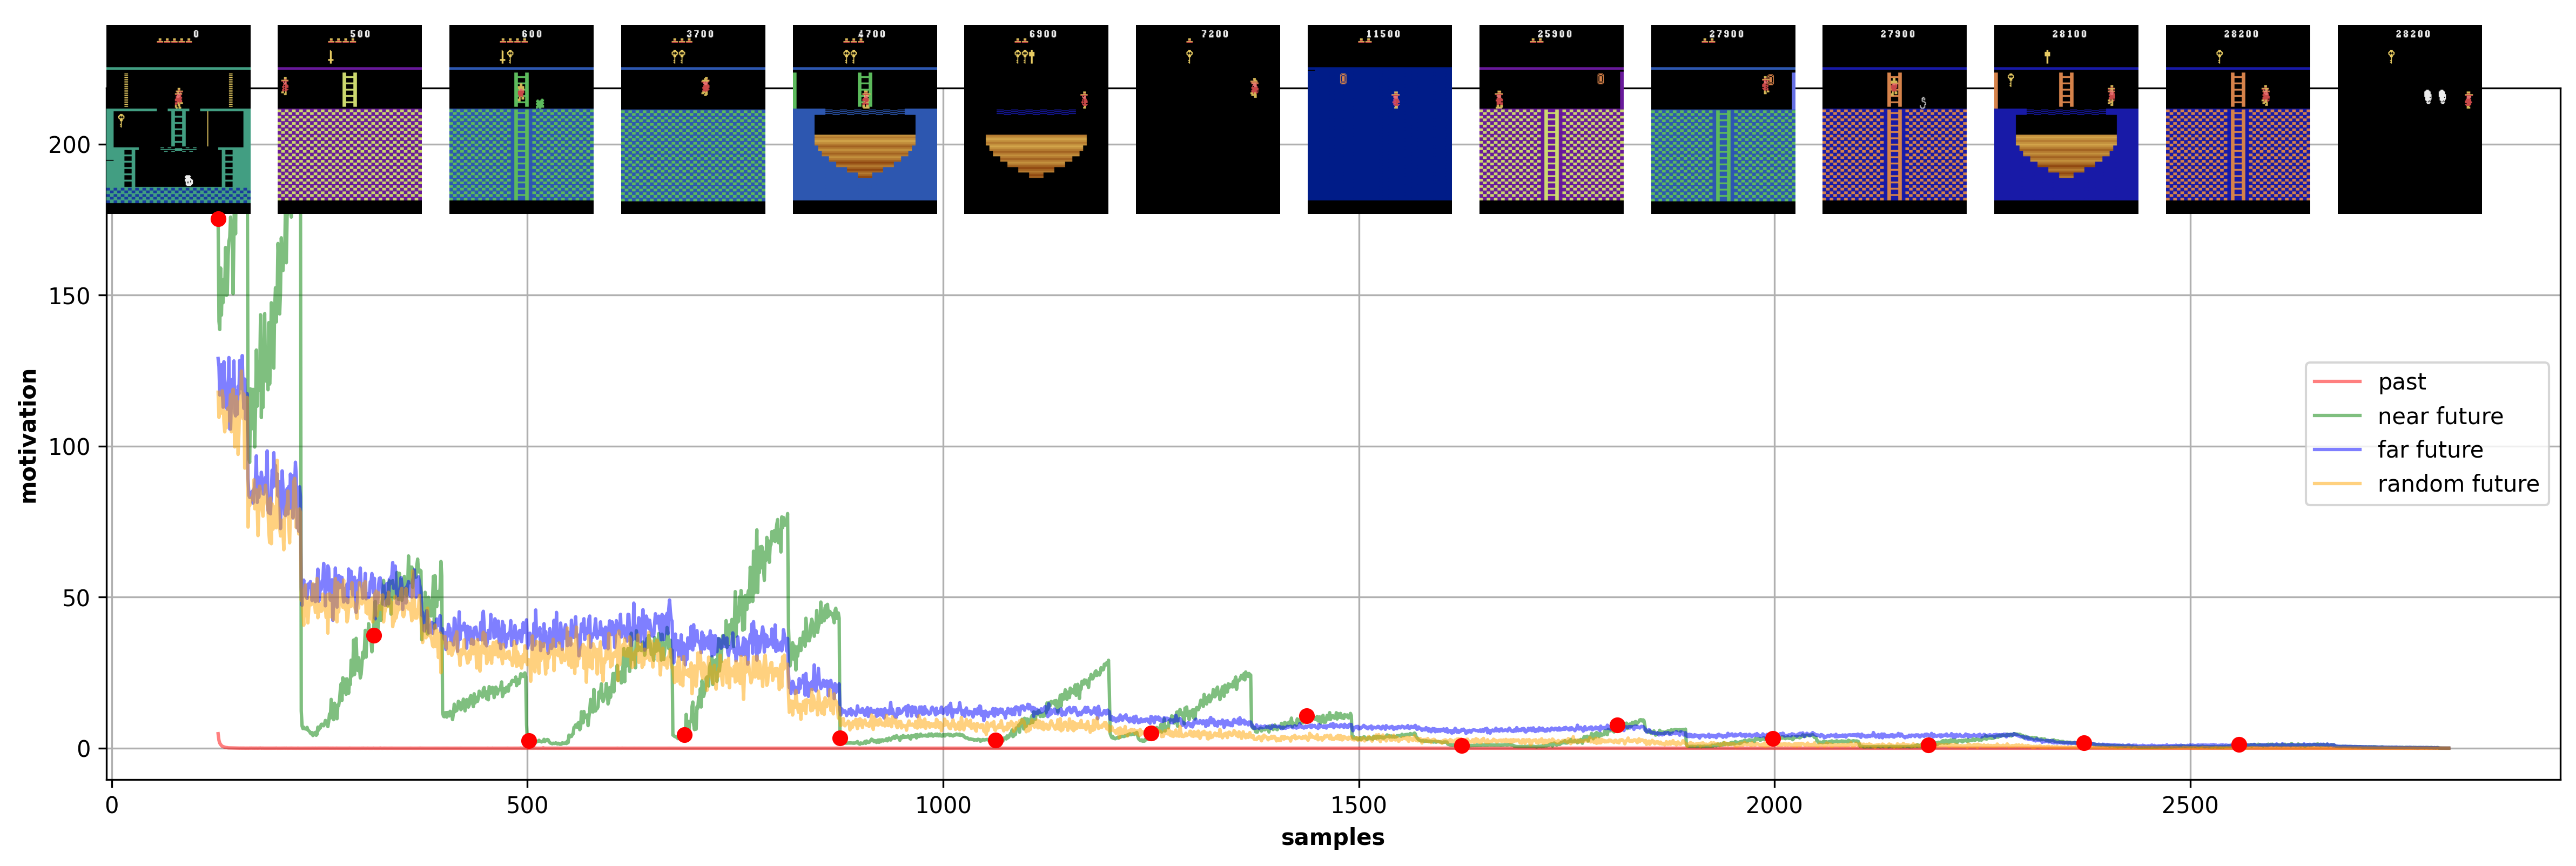
\includegraphics[width=12cm]{fig/results/novelty_detection/rnd_result_summary.png}
    \caption{RND}
    \label{fig:nov_rnd_result_summary}
   \end{subfigure}
  \\
  \begin{subfigure}{1.0\textwidth}
    \centering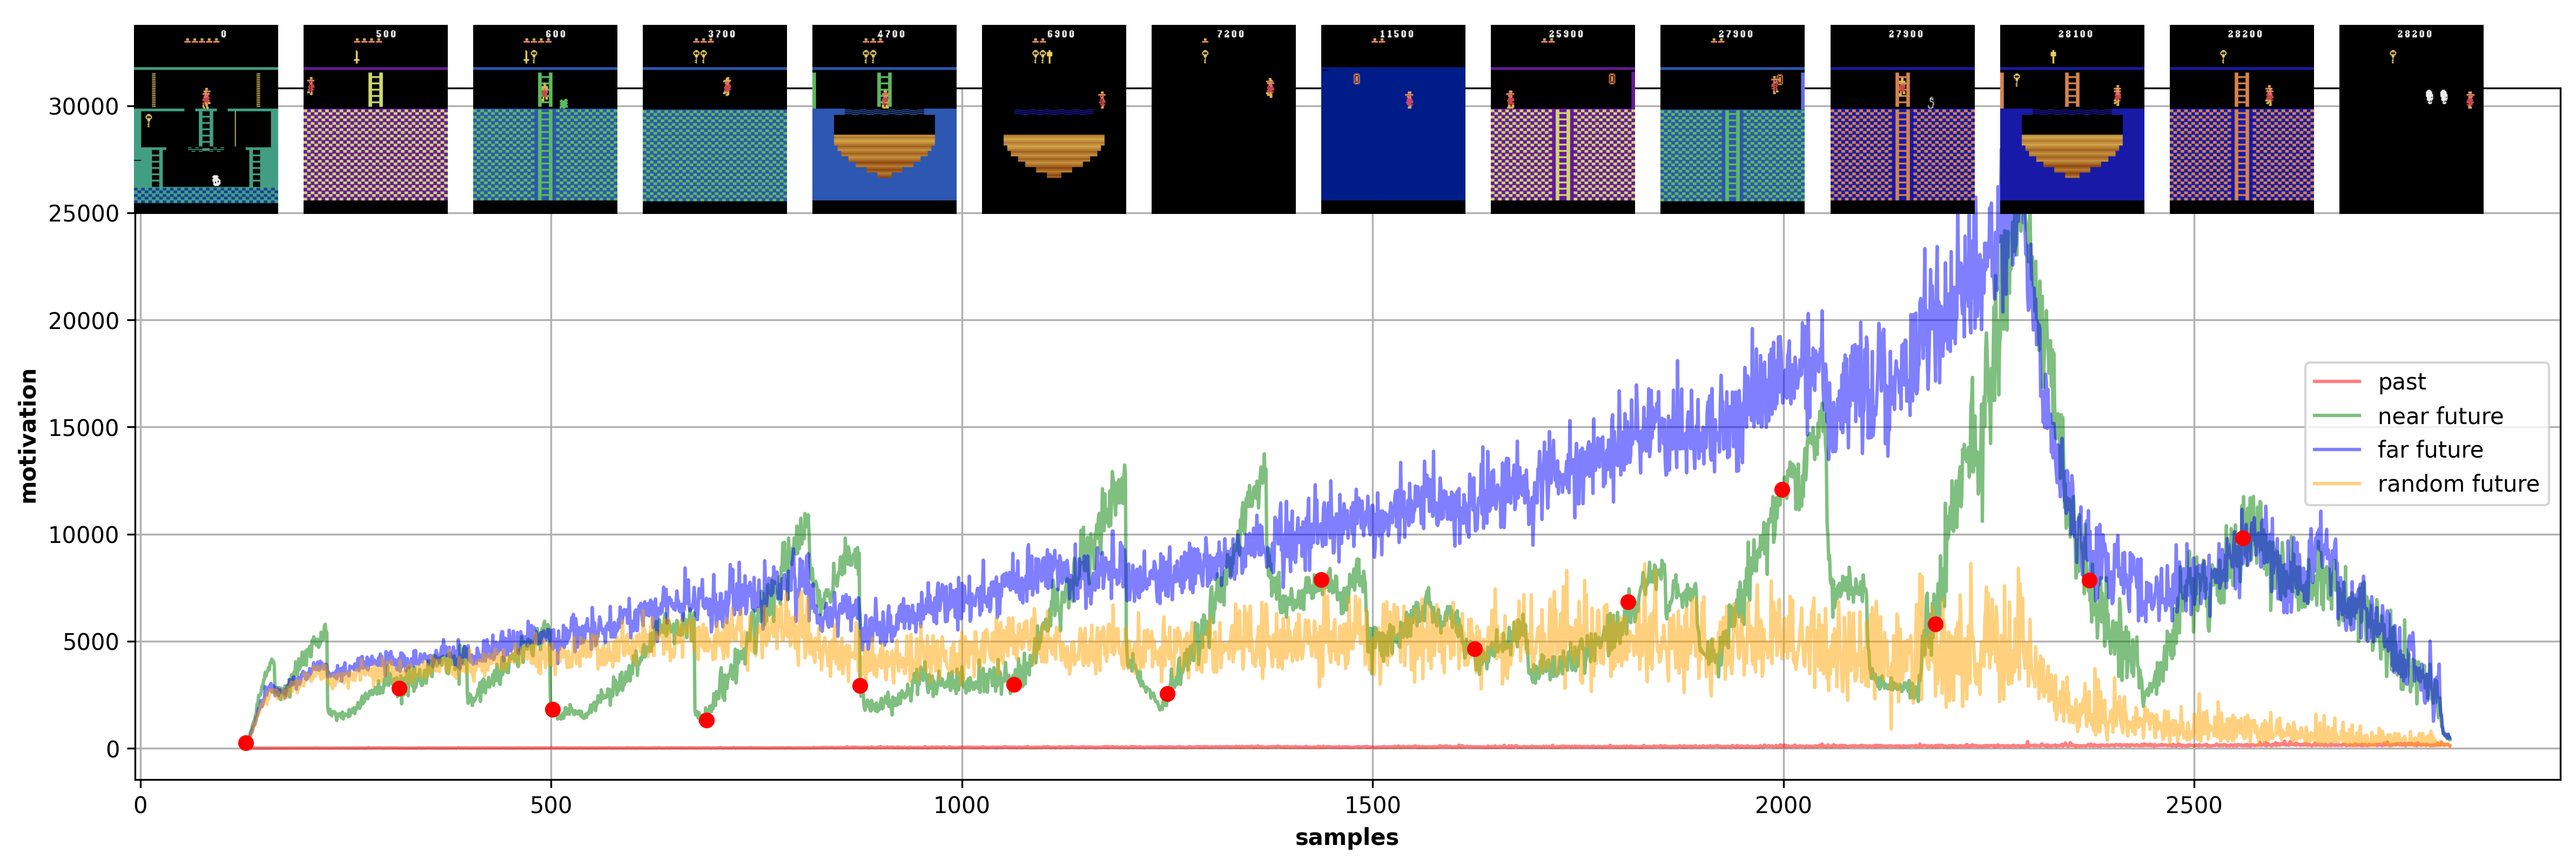
\includegraphics[width=12cm]{fig/results/novelty_detection/cnd_nce_summary.png}
    \caption{SND-STD}
    \label{fig:nov_nce_result_summary}
   \end{subfigure}
  \\
  \begin{subfigure}{1.0\textwidth}
    \centering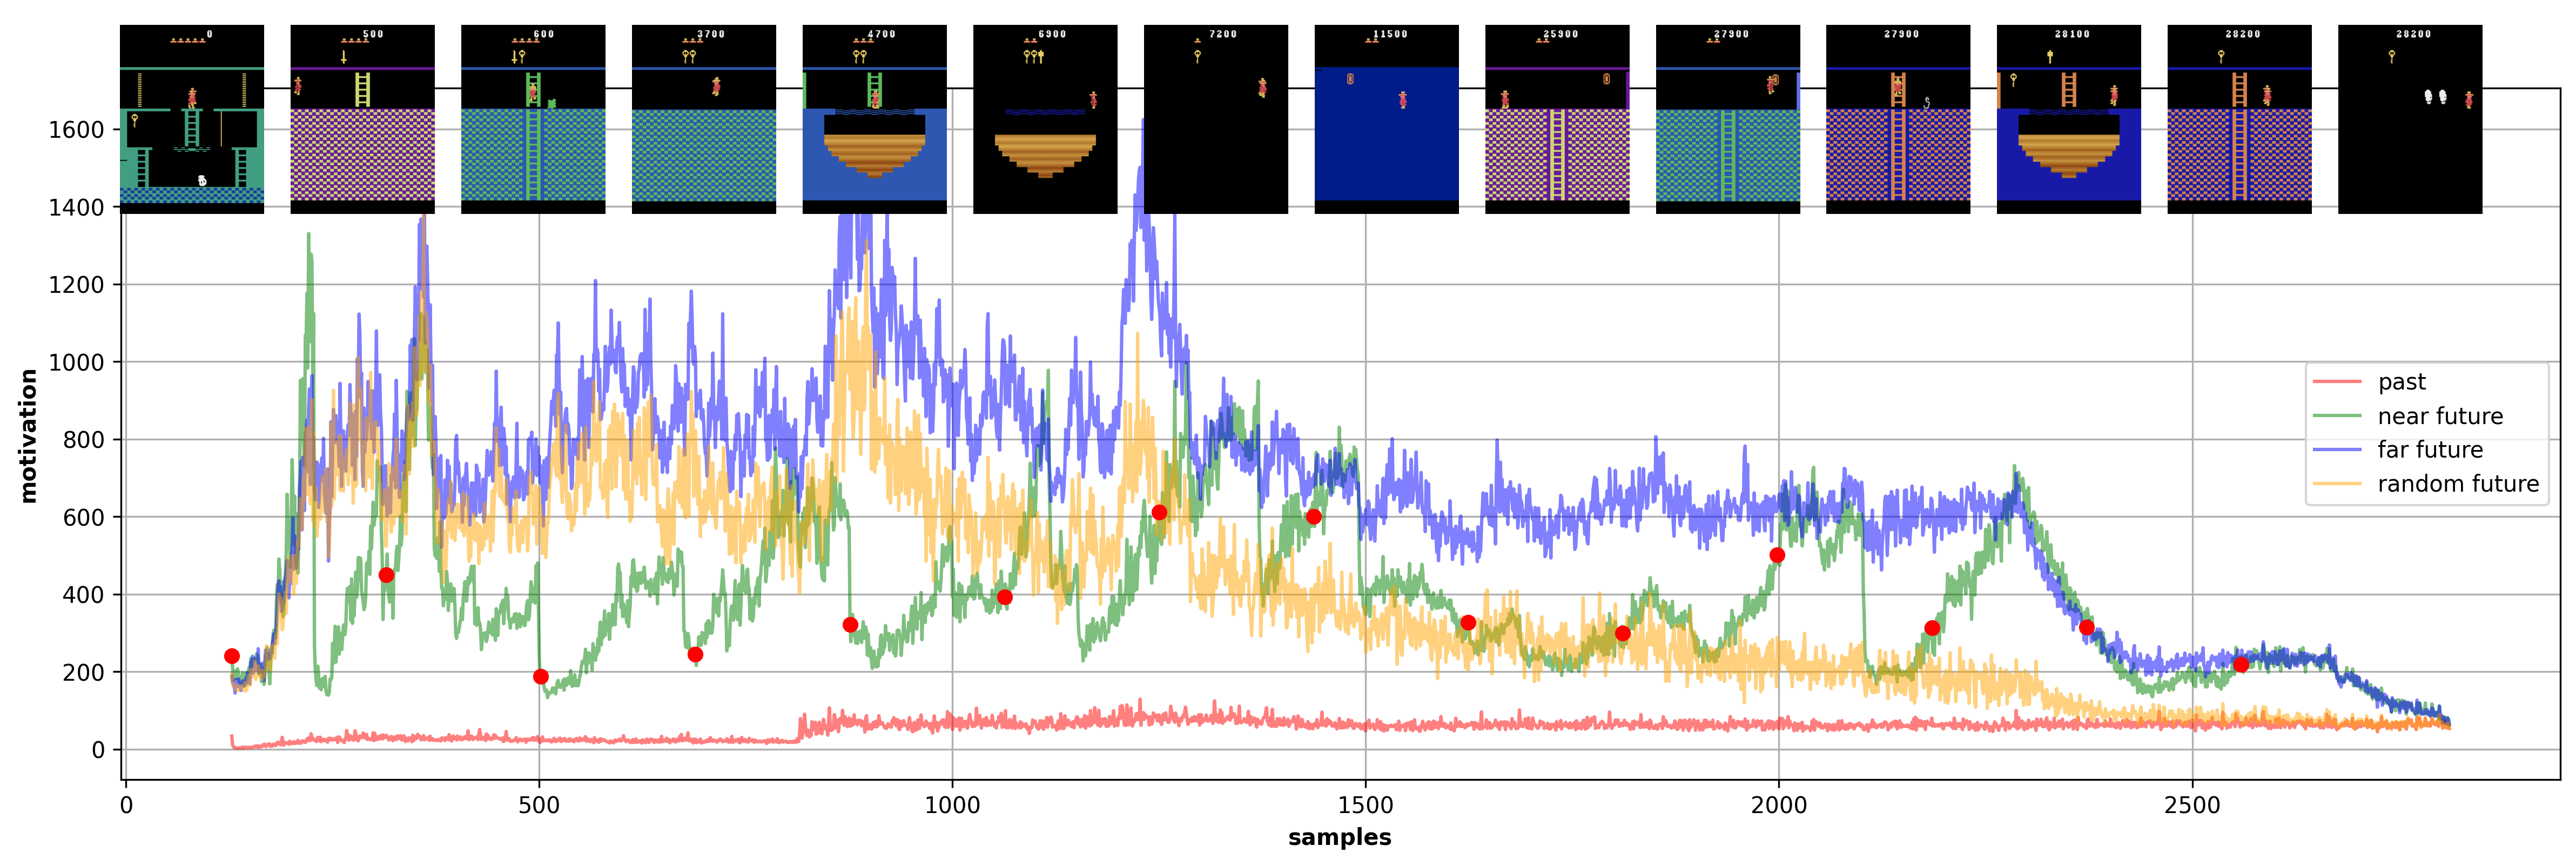
\includegraphics[width=12cm]{fig/results/novelty_detection/cnd_msev_result_summary.png}
    \caption{SND-V}
    \label{fig:nov_mse_result_summary}
   \end{subfigure}
  \\
  \begin{subfigure}{1.0\textwidth}
    \centering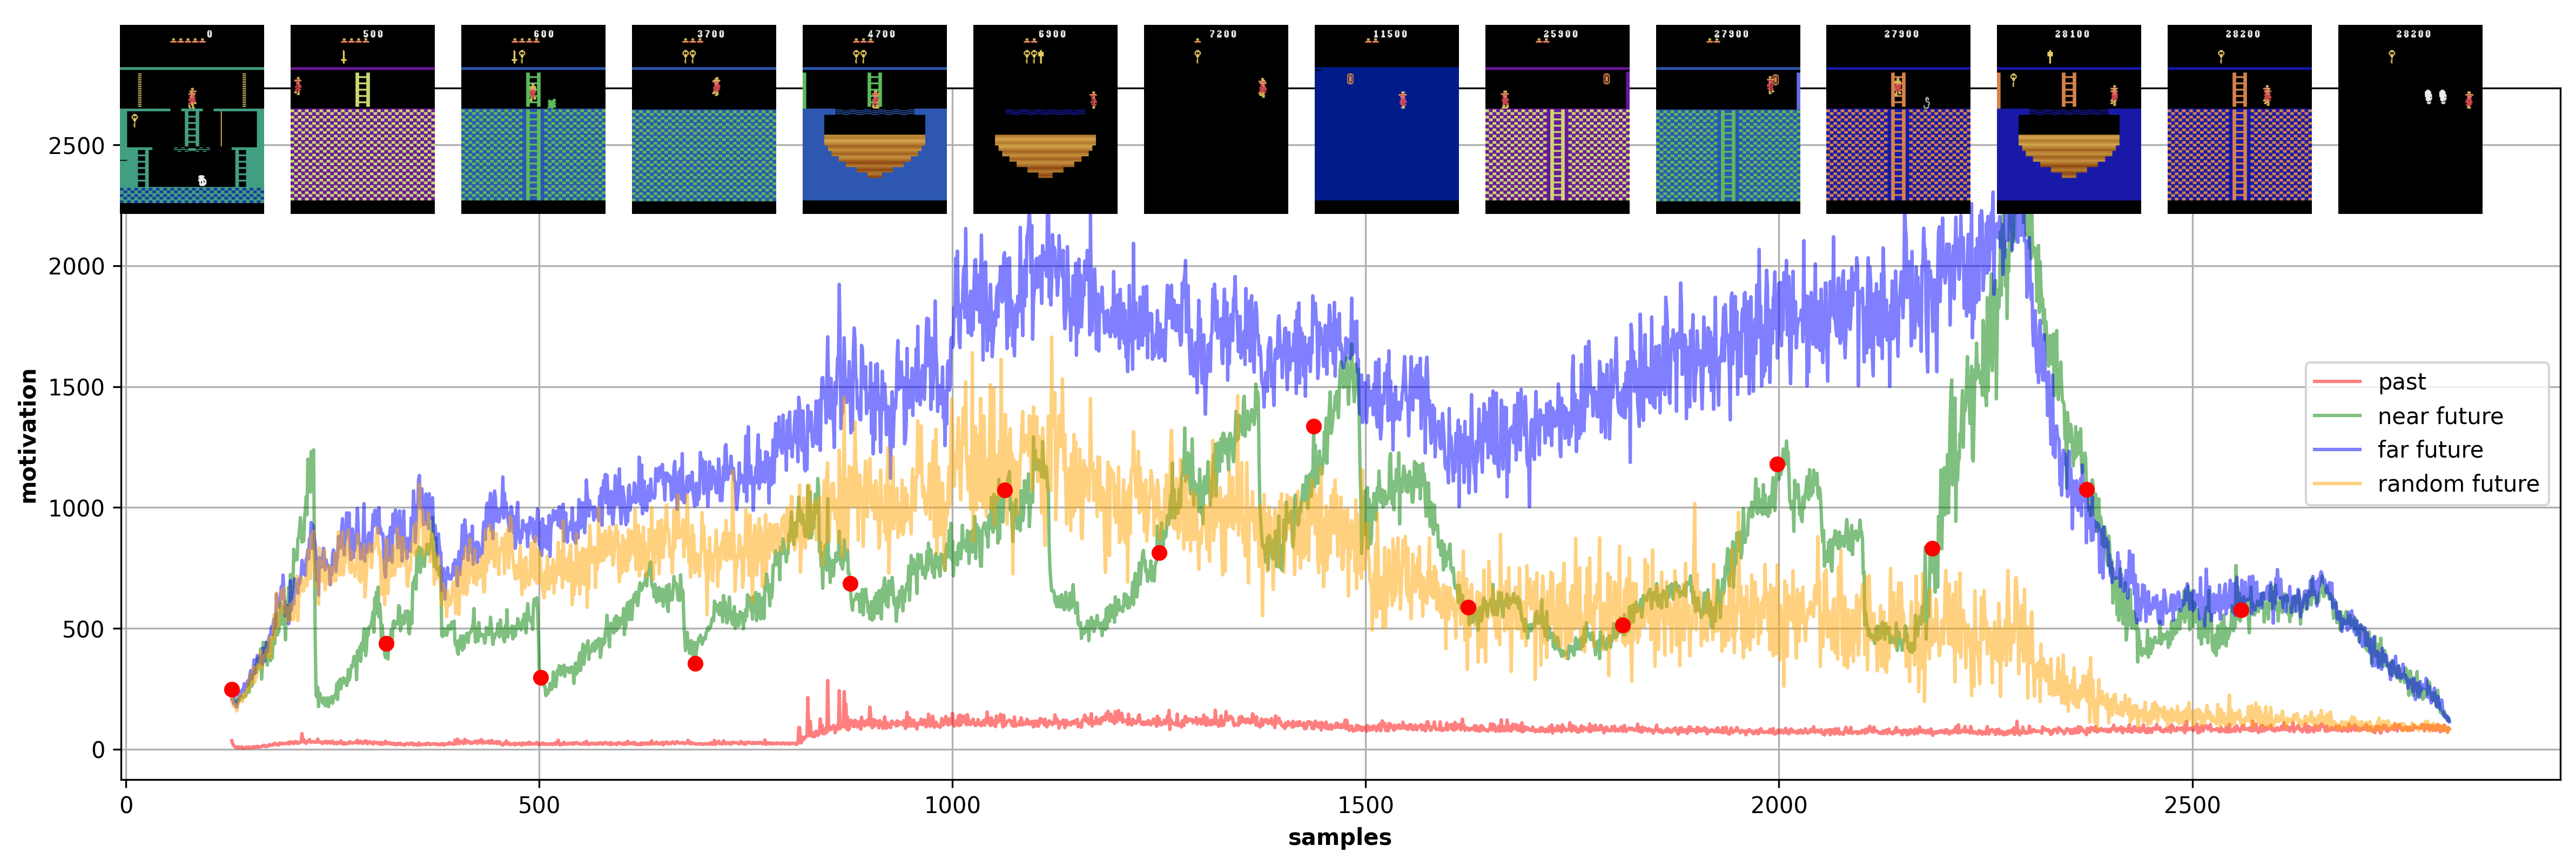
\includegraphics[width=12cm]{fig/results/novelty_detection/cnd_vicreg_result_summary.png}
    \caption{SND-VIC}
    \label{fig:nov_vicreg_result_summary}
   \end{subfigure}
\caption{Novelty detection for different regularisation losses as react on different future window. The states were collected on Montezuma's Revenge with our best agent, red dots correspond to state examples above.}
\end{figure*}

We can visualise learned feature vectors $Z$ in 2D using t-SNE method \citep{tSNE2008}. Figure~\ref{fig:cnd_feature_space} shows resulted features of trained $\Phi^{\rm T}$ on Atari Montezuma's revenge. The randomly initialised trained network (the same as in \cite{burda2018exploration} in Figure~\ref{fig:target_features_random}) can well distinguish between different rooms, however within the room the variance is low, pointing to the lack of exploration abilities. On the other hand, self-supervised regularized target model in Figure~\ref{fig:cnd_feature_space} provides much larger variance of features, which provides more sensitive novelty detection signal.

The main goal of the analysis was to find out the differences (not only visually) between the individual spaces of features, to describe them with some quantities and to find a possible connection with the performance of the algorithm and the mentioned quantities. From the set of examined models for one environment, we always selected the model with the highest obtained reward and generated 10,000 samples of input states by running it in the environment. Subsequently, each model generated feature vectors for a sample of previously collected input states. Thus, we obtained feature space samples $Z$ of each model. Then, using principal component analysis (PCA), we found the linear envelope of the high-dimensional manifold that forms the feature space. We examined the mean value and especially the variance of the feature vectors and also the eigenvalues obtained using PCA, which at least indicate something about the basic shape of the feature space (i.e. the sizes of the individual dimensions).

The results of this analysis are shown in Fig.~\ref{fig:cnd_analysis} and Tab.~\ref{tab:analysis1}. For the evaluation, we decided to use the following parameters: mean value and standard deviation of the $L_{2}$-norm of features, 25th, 50th, 75th and 95th percentiles of eigenvalues to obtain a rough representation of stretching of the feature space in individual dimensions.
It can be seen that in almost all cases the RND target model has smaller eigenvalues than the SND models. This can also be seen in the $L_2$-norm values that the entire RND feature space seems to have a smaller volume compared to the SND feature space. 
We can see that RND and SND-STD are similar in shape. Their curve has a convex shape, with SND-STD having more stretched dimensions. SND-V and SND-VIC also have similarly concave shapes but SND-V stretches only about half of the available dimensions and then usually falls more steeply. The shape of SND-VIC curve is ensured by the variance (eq.~\ref{eq:sndvic1}) and covariance (eq.~\ref{eq:sndvic2}) components of its loss function. The missing decorrelation term in the SND-V loss function (eq.~\ref{eq:sndv2}) results in an uneven stretching of the dimensions.

In contrast, the shape of the SND-STD curve is convex and the dimensions are used unevenly. After these analyses, we tried to improve the variance within the dimensions by adding a regularization term (eq.~\ref{eq:sndstd5}) which tried to maximize the variance within the feature vector. However, such a term had an expansive effect on the feature space and it was not possible to give it much weight, because the loss function (eq.~\ref{eq:sndstd3}) of the ST-DIM algorithm itself has an expansive effect, and the addition of another expansive term led to problems with the uncontrolled expansion of the feature space. 
Despite the small influence of the variance component of the loss function, the performance of SND-STD improved and it helped prevent agents from getting stuck in certain cases. If we compare RND and SND-STD feature spaces (in terms of eigenvalues) they look similar, but the latter model was able to achieve better results in 7 out of 9 environments. Our findings show that when training the target model, it is important to enforce the decorrelation of features and the equal use of all dimensions of the feature space. Such a model seems to be relatively robust and sufficiently sensitive to novelty.

Interestingly, for Pitfall task (not shown in Figure~\ref{fig:cnd_analysis}), despite their failure, our methods still tried to take advantage of the feature space dimensions. 
From the analysis of the trained agents, we saw that they were able to explore several rooms, but in each there were enough moving objects that made the given state space rich and thus made it difficult to train the learned model, which led to a very slow decrease of the internal reward (we observed a similar behavior after short training sessions in other environments). We assume that with a larger number of training steps, the agent would eventually be able to reach the reward.

Another approach for different regularisation losses is understanding its time evaluation and the ability to provide large IM signal for previously unseen states. For the purpose of exploration, the most important is the ability to detect near future states, which are very close to already seen ones. We collected a set of 2700 states, from our best agent playing Montezuma's Revenge. During the experiment, we trained the IM modules only on past data, and tested on future data. The testing batch was selected from the following 4 time horizons, with respect to the agent being in step $n$, and testing batch indices $m$:
\begin{enumerate}
    \item past: already seen states, $m<n$
    \item near future: $n < m < n+128$ steps in the future
    \item far future: $m > n$
    \item random: any batch from the set
\end{enumerate}

We hypothesised that the Random Network distillation provides a sufficient signal only at the beginning of learning. Converging to zero leads to limited exploration abilities. This degradation corresponds to our results in Figure~\ref{fig:nov_rnd_result_summary}.
On the other hand, continuously updated target models can provide useful signals for the entire run. The corresponding results are displayed in Figures \ref{fig:nov_nce_result_summary}, \ref{fig:nov_mse_result_summary}, and \ref{fig:nov_vicreg_result_summary}. On all three losses, the intrinsic motivation is much higher for non-seen states, and not converging into zero. The strong peeks for near future correspond to new rooms finding. The self supervised regularisation prevents collapsing motivation signal to zero. 
This insight gives us requirements for exploration signal.
For future research we got also simple methodology for testing exploration abilities, without training whole RL agent which can be time consuming. 


%%%%%%%%%%%%%%%%%%%%%%%%%%%%%%%%%%%%%%%%%%%%%%%%%%%%%%%%%%%%%%%%%%%%%%%% CHAPTER 5
\section{Discussion}
\label{sec:discussion}

We introduced a class of internal motivation algorithms, based on distillation error as a novelty indicator (SND), where the target model is trained using self-supervised learning. We adapted three existing self-supervised methods for this purpose and experimentally tested them on a set of environments that are considered difficult to explore.
The proposed variants have been shown to eliminate the identified shortcomings of the RND model -- the need for good initialization, low variance of intrinsic reward on different states and the loss of the motivational signal caused by the adaptation of the learning network.

In the experiments, we tested the overall performance of the agents in 10 environments. With the exception of one environment, it was confirmed that the SND algorithms achieved better results than other methods with which we compared them. For the Atari environments, we also evaluated the achieved game scores so that they could be compared with other published models that we did not include in in this work. Also from the point of view of the SND score, the models dominated the compared models.

In the analytical part, we focused on deeper understanding of the SND methods. We used a geometric approach trying to capture, at least in rough outlines, the properties of feature spaces. A comparison between a randomly initialized feature space and a feature space formed using one of the SND algorithms shows the correctness of our assumptions that self-supervised algorithms can distinguish even subtle differences within the state space. This turned out to be one of the weaknesses of the RND algorithm, which, while being good at distinguishing between sufficiently different states (e.g. different rooms in Montezuma's Revenge), it placed similar states close to each other in the feature space, making the work of the learned model easier. In the experiments, we thus observed a decrease in the standard deviation of the average intrinsic reward per episode, which meant that most of the visited states generated a similar reward.


We experimented with different target model architectures, different augmentations and intrinsic reward scaling. We found that the target model using ELU activation and only one fully connected layer with the learned model with three hidden layers performs the best. 
From the tested augmentations (noise, random tile masking, random convectional filter), we found the best performance for a combination of uniform noise with random tiles masking. As a questionable augmentation remains random down sampling and up sampling back, which could help remove noise while preserving representative information in the state vectors. We suggest to investigate this idea for next research.
The scaling of intrinsic reward shows big sensitivity to this parameter. The best working value was $0.5$, however we think this value should be optimized separately for each specific environment.  

We did not specifically investigate the robustness of SND methods with regard to the initialization of the target model (which was again a problem with RND). We assume that self-supervised learning algorithms can cope with a poorly initialized model to a certain extent, but from the training experience we found that it is better to initialize the target models of SND-STD and SND-VIC to small values ($gain = 0.5$) and letting it expand itself while SND-V was initialized like RND to higher values ($gain = \sqrt{2}$).

Our experiments revealed that if the ST-DIM algorithm works on an incomplete dataset that takes on new samples (the authors probably did not test it in such conditions), there is an instability and an exponential increase of activity in the feature space at certain moments. This is related to the use of cross-entropy loss function in its core (which does not limit the values of inputs, logits), where derivatives can reach large values and subsequently inflate the entire feature space. During the development of the model, it turned out that it is best to minimize the $L_2$-norm of logits that enter the cross-entropy. In addition, we tried to maximize the entropy of the distributions generating the respective logits and minimize the $L_2$-norm of global features. However, both described approaches failed to sufficiently stabilize the algorithm.

We also compared the effect of state preprocessing on the performance of the SND-STD model. It turned out that the state preprocessing is not necessary since it has no significant effect on the agent's performance.

We also performed an analysis of novelty detection abilities of selected methods. After comparison with RND as a baseline, we can conclude that this baseline suffers from an IM-based reward vanishing problem. After adding the regularisation to the target model, much better features were obtained, with significant change compared to the baseline. Intrinsic reward vanishing disappears for all the tested losses. This is cross-validated also on $t$-SNE features visualisation, where regularised features yield much higher variance, which means larger sensitivity to novelty.

Based on the presented results, we can conclude that self-supervised learning methods are definitely promising in the creation of novelty detectors, which can be successfully used from the point of view of intrinsic motivation and improve the agent's exploration. A direct extension of SND methods will be the merging of the target model with the model to which the actor and critic are connected. We have already done some pilot research in this direction and it seems to be a feasible task. This would greatly optimize the entire model and speed up its training in terms of computing time.
At the same time, we think that this approach can be an inspiration for a new class of algorithms that will specialize in creating feature mapping capturing the relationship of the environment to the agent itself, since current self-supervised methods are agnostic to these relationships.

%%%%%%%%%%%%%%%%%%%%%%%%%%%%%%%%%%%%%%%%%%%%% BIBLIOGRAPHY
\vspace{3,16314mm}
%\nocite{*}
\bibliographystyle{apalike}  %preco nie toto?
%\bibliographystyle{elsarticle-num}
\bibliography{references}
 

\end{document}
